% !BIB TS-program = biber
% !BIB program = biber
\documentclass[a4paper,12pt]{book}
\usepackage[utf8]{inputenc}
\usepackage{lmodern,textcomp}
\usepackage{graphicx}
\usepackage{booktabs}
\usepackage{tabularx}
\usepackage{tikz}
\usepackage{pgfplots}
\usepackage{url}
\usepackage{wrapfig}
\usepackage{newfloat}

\usepackage{tcolorbox}

\usepackage{codex}

\tcbuselibrary{skins,breakable,xparse,raster}

\usepackage[scaled]{beramono}
\usepackage[T1]{fontenc}

\usepackage[
backend=biber,
style=apa,
natbib=true,
sortlocale=en_US,
url=true, 
doi=true,
eprint=false
]{biblatex}
\addbibresource{references.bib}

%to make line breaks possible at more parts within \texttt
\renewcommand{\texttt}[1]{%
	\begingroup
	\ttfamily
	\begingroup\lccode`~=`/\lowercase{\endgroup\def~}{/\discretionary{}{}{}}%
	\begingroup\lccode`~=`[\lowercase{\endgroup\def~}{[\discretionary{}{}{}}%
	\begingroup\lccode`~=`.\lowercase{\endgroup\def~}{.\discretionary{}{}{}}%
	\begingroup\lccode`~=`(\lowercase{\endgroup\def~}{(\discretionary{}{}{}}%
	\catcode`/=\active\catcode`[=\active\catcode`.=\active\catcode`(=\active
	\scantokens{#1\noexpand}%
	\endgroup
}
        
\usepackage[colorinlistoftodos]{todonotes}


\usepackage{listings}
\lstset{
	basicstyle=\tiny\ttfamily,
	columns=flexible,
	breaklines=true,
	%stepsize=1,
}

\definecolor{darkblue}{rgb}{0,0,0.3}
\lstdefinestyle{r}{language=R,
  showstringspaces=false,
  stringstyle=\color{darkblue},
  morekeywords={select,filter,rename},
  numbers=left,
	numberstyle=\tiny\color{gray},
        numbersep=4pt,
}
\lstdefinestyle{py}{language=python,
  showstringspaces=false,
  stringstyle=\color{darkblue},
  morekeywords={select,filter,rename},
  numbers=left,
	numberstyle=\tiny\color{gray},
        numbersep=4pt,
}
\lstdefinestyle{out}{language={},
  showstringspaces=false,
  stringstyle=\color{darkblue},
  morekeywords={select,filter,rename},
}

\lstnewenvironment{exampler}{\lstset{basicstyle=\scriptsize\ttfamily,
		columns=flexible,
		breaklines=true,
		numbers=left,
		%stepsize=1,
		numberstyle=\tiny}}{}

\lstnewenvironment{ex_r_out}{\lstset{basicstyle=\scriptsize\ttfamily,
		columns=flexible,
		breaklines=true, 
		numbers=left,
		%stepsize=1,
		numberstyle=\tiny,
		backgroundcolor=\color[rgb]{0.3,0.3,1}}}{}

\lstnewenvironment{ex_r_in}{\lstset{basicstyle=\scriptsize\ttfamily,
		columns=flexible,
		breaklines=true,
		numbers=left,
                showlines=true,
		%stepsize=1,
		numberstyle=\tiny,
		backgroundcolor=\color[rgb]{0.5,0.5,1}}}{}

\lstnewenvironment{ex_py_out}{\lstset{basicstyle=\scriptsize\ttfamily,
		columns=flexible,
		breaklines=true,
		numbers=left,
		%stepsize=1,
		numberstyle=\tiny,
		backgroundcolor=\color[rgb]{0,0.6,.25}}}{}

\lstnewenvironment{ex_py_in}{\lstset{basicstyle=\scriptsize\ttfamily,
		columns=flexible,
		breaklines=true,
		numbers=left,
		%stepsize=1,
                showlines=true,
		numberstyle=\tiny,
		backgroundcolor=\color[rgb]{0.2,0.6,0.5}}}{}

\lstnewenvironment{examplepy}{\lstset{basicstyle=\scriptsize\ttfamily,
		columns=flexible,
		breaklines=true,
		numbers=left,
		%stepsize=1,
		numberstyle=\tiny,
		%backgroundcolor=\color[rgb]{.7,.7,.7}}}{}
		backgroundcolor=\color[rgb]{0,.6,.25}}}{}

\newcommand{\refsec}[1]{Section~\ref{sec:#1}}
\newcommand{\reffig}[1]{Figure~\ref{fig:#1}}
\newcommand{\reftab}[1]{Table~\ref{tab:#1}}
\newcommand{\refex}[1]{Example~\ref{ex:#1}}

\newcommand{\code}[1]{\texttt{#1}}

\newcommand{\note}[1]{\noindent\fbox{
  \begin{minipage}{\textwidth}
    \textbf{Note:} #1
  \end{minipage}}}


\lstnewenvironment{terminal}{\lstset{basicstyle=\scriptsize\ttfamily,
		columns=flexible,
		breaklines=true,
		numbers=left,
		%stepsize=1,
		numberstyle=\tiny,
		backgroundcolor=\color[rgb]{.7,.7,.7}}}{}



\newcommand{\rex}[1]{%
\begin{tcolorbox}[colback=red!5!white,colframe=red!75!black,title=R code]
  \lstinputlisting[style=r]{#1.r}
  \tcbsubtitle{Output}
  \lstinputlisting[style=out]{#1.r.out}
\end{tcolorbox}}

\newcommand{\pyex}[1]{%
\begin{tcolorbox}[colback=red!5!white,colframe=red!75!black,title=Python code]
  \lstinputlisting[style=py]{#1.py}
  \tcbsubtitle{Output}
  \lstinputlisting[style=out]{#1.py.out}
\end{tcolorbox}}

\newtcolorbox{rbox}[1]{#1}

\newcommand{\rpyex}[2]{
  \begin{example}
  \begin{tcbraster}[raster columns=2,raster equal height=rows,raster valign=top]
    \rex{#1}
    \pyex{#1}
  \end{tcbraster}
  \caption{#2}
  \end{example}
}

\newcommand{\rexcode}[1]{%
\begin{tcolorbox}[colback=red!5!white,colframe=red!75!black,title=R code]
  \lstinputlisting[style=r]{#1.r}
\end{tcolorbox}}

\newcommand{\pyexcode}[1]{%
\begin{tcolorbox}[colback=red!5!white,colframe=red!75!black,title=Python code]
  \lstinputlisting[style=py]{#1.py}
\end{tcolorbox}}


\newcommand{\rpyexcode}[2]{
  \begin{example}
  \begin{tcbraster}[raster columns=2,raster equal height=rows,raster valign=top]
    \rexcode{#1}
    \pyexcode{#1}
  \end{tcbraster}
  \caption{#2}
  \end{example}
}


%\includeonly{ch_data_wrangling/ch_data_wrangling}
\includeonly{chapter06/chapter06, ch_data_wrangling/ch_data_wrangling}

\begin{document}

\author{Wouter van Atteveldt, Damian Trilling, Carlos Arcila Calder\'on}
\title{Computational Analysis of Communication}
\date{\today}

\frontmatter
\maketitle
\tableofcontents

\mainmatter

\part{Getting Started}

\setcounter{chapter}{1}
\chapter{Fun with Data!}
\label{chap:fundata}

\input{chapter02/colab}
\section{Fun with tweets}

The goal of this chapter is to showcase how you can use R or Python to quickly and easily
run some impressive analyses of real world data.
For this purpose, we will be using a data set of tweets about the COVID pandemic that is
engulfing much of the world at the time this book is written.
Of course, tweets are probably only representative for what is said on Twitter,
but the data are (semi-)public and rich, containing text, location, and network characteristics.
This makes them ideal for exploring the many ways in which we can analyze and visualize information
with Python and R. 

\refex{funtweets} shows how you can read this data set into memory using a single command.
Note that this does not retrieve the tweets from Twitter itself, but rather downloads
our cached version of the tweets.
In \refchap{scraping} we will show how you can download tweets and location data yourself, but to make sure
we can get down to business immediately we will start from this cached version. 

\begin{ccsexample}
  \doublecodex{chapter02/tweets}
\codex[caption=Output]{chapter02/tweetsb.r.out}
\caption{Retrieving cached tweets about COVID}\label{ex:funtweets}
\end{ccsexample}

As you can see, the dataset contains almost ten thousand tweets, listing their
sender, their location and language, the text, the number of retweets, and whether it was a reply (retweet).
You can read the start of the three most retweeted messages, which contain one (political) tweet from India
and two seemingly political and factual tweets from the United States.

\paragraph{My first bar plot} Before diving into the textual, network, and geographic data in the data set,
let's first make a simple visualization of the date at which the tweets are posted.
\refex{funtime} does this in two steps:
First, the number of tweets per hour is counted with an aggregation command.
Next, a bar plot is made of this calculated value with some options to make it look relatively clean and professional.
If you want to play around with this, you can for example try to plot the amount of tweets per language,
or create a line plot instead of a bar plot. 
For more information on visualization, please see \refchap{eda}.
See \refchap{datawrangling} for an in-depth explanation of the aggregation command. 

\pyrex[caption=Barplot of tweets over time,input=both,output=r,format=png]{chapter02/funtime}

\section{Fun with textual data}

\paragraph{Corpus Analysis} Next, we can analyze which hash tags are most frequently used in this data set.
\refex{funcloud} does this by creating a \concept{document-term matrix} using the package \pkg{quanteda} (in R)
or \sklearn (in Python).
The code shows a number of steps that are made to create the final results, each of which represent
researcher choices about which data to keep and what to discard as noise.
In this case,  we select English tweets, convert text to lower case, remove stop words, and keep only words that start with \#,
while dropping words starting with \verb+#corona+ and \verb+#covid+.
To play around with this example,
see if you can adjust the code to e.g. include all words or only at-mentions instead of the hash tags
and make a different selection of tweets, for example Spanish language tweets or only popular (retweeted) tweets.
Please see \refchap{dtm} if you want to learn more about corpus analysis,
and see \refchap{datawrangling} for more information on how to select subsets of your data.

\pyrex[caption=My First Tag Cloud,input=both,output=r,format=png]{chapter02/funcloud}

\paragraph{Topic Model}
Where a word cloud (or tag cloud) shows which words occur most frequently,
a \concept{topic model} analysis shows which words co-occur in the same documents.
Using the most common topic modeling algorithm, Latent Dirichlet Allocation or LDA,
\refex{funlda} explores the tweets by automatically clustering the tags selected earlier into 10 \emph{topics}.
Topic modeling is non-deterministic -- if you run it again you can get slightly different topics,
and topics are swapped around randomly as the topic numbers have no special meaning.
By setting the computer's \concept{random seed} you can ensure that if you run it again you get the same results.
As you can see, some topics seem easily interpretable (such as topic 6 about economic consequences,
and topic 7 about masks and prevention), it is always recommended to inspect the clustered documents
and edge cases in addition to the top words (or tags) as shown here.
You can play around with this example, for example by using a different selection of words
(modifying the code in \refex{funcloud}) or changing the number of topics.
You can also change (or remove) the random seed and see how running the same model multiple times give different results. 
See \refsec{unsupervised} for more information about fitting, interpreting, and validating topic models.

\pyrex[caption=Topic Model of the COVID tags,input=both,output=r,format=table]{chapter02/funlda}

\section{Fun with visualizing geographic information}
For the final set of examples, we will use the location information contained in the twitter data.
This information is based on what twitter users enter into their profile, and as such it is incomplete and noisy
with many users giving a nonsensical location such as `Ethereally here' or not filling in any location at all.
However, if we assume that most users that do enter a proper location (such as Lahore or Florida in the top tweets displayed above),
we can use it to map where most tweets are coming from.

The first step in this analysis is to resolve a name such as `Lahore, Pakistan' to its geographical coordinates (in this case, about 31 degrees north and 74 degrees east). This is called geocoding, and both Google maps and Open Street Maps can be used
to perform this automatically.
As with the tweets themselves, we will use a cached version of the geocoding results here so we can proceed directly.
At the end of this chapter we will show the code that was used to create this file so you can play around with it as well. 

\refex{funmap} shows how this data can be used to create a map of twitter activity.
First, the cached user data is retrieved, showing the correct location for Lahore but also
illustrating the noisiness of the data with the location `Un peu partout'.
Next, this data is \concept[joining]{joined} to the twitter data, so the coorinates are filled in where known.
Finally, we plot this information on a map, showing tweets with more retweets as larger dots.
See \refchap{eda} for more information on visualization.

\pyrex[caption=Location of COVID tweets,input=both,output=r,format=png]{chapter02/funmap}


\paragraph{Combining textual and structured information}
Since we know the location of a subset of our tweet's users,
we can differentiate between e.g. American, European, and Asian tweets.
\refex{funcompare} creates a very rough identification of North American tweets,
and uses that to compute the relative frequency of words in those tweets compared to the rest.
Not surprisingly, those tweets are much more about American politics, locations, and institutions.
The other tweets talk about UK politics but also use a variety of names to refer to the pandemic.
To play around with this, see if you can isolate e.g. Asian or South American tweets,
or compare Spanish tweets from different locations.

\pyrex[caption=Corpus comparison: North American tweets vs. the rest,input=both,output=r,format=png]{chapter02/funcompare}

% TODO CITE THIS FOR PYTHON EXAMPLE? Gallagher, R. J., Frank, M. R., Mitchell, Lewis, Schwartz, A. J., Reagan, A. J., Danforth, C. M., Dodds, P. S.. (2020). Generalized Word Shift Graphs: A Method for Visualizing and Explaining Pairwise Comparisons Between Texts. arXiv preprint 2008.02250.

\section{Fun with networks}

Twitter, of course, is a social network as well as a microblogging service:
users are connected to other users because they follow each other and retweet and like each others' tweets.
Using the \verb+reply_to_screen_name+ column, we can inspect the retweet network contained in the COVID tweet data set.
\refex{fungraph} first uses the data summarization commands from \tidyverse\ (R) and \pandas\ (Python) to
create a data frame of connections or \concept{edges} listing how often each user retweets each other user.
The second code block shows how the \pkg{igraph} package is used to convert this edge list into a graph.
From this graph, we select only the largest connected component and use a clustering algorithm to analyze which
nodes (users) form cohesive subnetworks.
Finally, a number of options are used to set the color and size of the edges, nodes, and labels,
and the resulting network is plotted.
As you can see, the central node is Donald Trump, who is retweeted by a large number of users,
some of which are then retweeted by other users.
You can play around with different settings for the plot options,
or try to filter e.g. only tweets from a certain language. 
You could also easily compute social network metrics such as centrality on this network,
and/or export the network for further analysis in specialized social network analysis software.
See \refchap{network} for more information on network analysis,
and \refchap{datawrangling} for the summarization commands used to create the edge list.

\begin{ccsexample}
  \doublecodex{chapter02/fungraph}
  \codexoutputtable{chapter02/fungraph.r}
  \doublecodex{chapter02/fungraphb}
  \codexoutputpng{chapter02/fungraphb.r}
\caption{Retweet nework in the COVID tweets}\label{ex:fungraph}
\end{ccsexample}

\paragraph{Geographic networks}
In the final example of this chapter, we will combine the geographic and network information to
show which regions of the world interact with each other.
For this, in \refex{fungeonet} we join the user information to the edges data frame created above twice:
once for the sender, once for the replied-to user.
Then, we adapt the earlier code for plotting the map by adding a line for each node in the network.
As you can see, users in the main regions (US, EU, India) mostly interact with each other,
with almost all regions also interacting with the US.

\pyrex[caption=Reply Network of Tweets,output=r,format=png]{chapter02/fungeonet}

\section{Using APIs}

The data used in the examples above were gathered using the APIs of Twitter and Open Street Map.
\refchap{scraping} will go into this in more detail, but it is shown in \refex{funapi} here as well for the sake of completeness
(and in case you are eager to have fun with those APIs).

Twitter is a popular data source for scientific analysis, mostly because it is relatively open, public, and easy to collect.
In R, we use \pkg{rtweet}, which will automatically ask you to log in to Twitter in a browser so it can obtain an API key
(remember that you might have to \verb|install.packages("rtweet")| if you haven't already done so).
After this, you can use the code in the second part of the example to lookup users and download tweets.
Note that this will only work if you run RStudio locally: if you use a jupyter notebook (e.g. in colab)
it will not be able to connect to your browser and you will have to obtain an API key yourself,
see \refchap{scraping} for more details. 

For the geocoding, we used Open Street Maps since it can be used without an API key.
In R, you need to install \pkg{tmaptools} and then you can use the \fn{geocode\_OSM} function as shown in \refex{funtmap}.
If you want to combine the user data with the tweets as in the examples above,
you can use the code in the last part of the example. 
Don't worry if you don't understand all of the code in that snippet yet,
after reading \refchap{datawrangling} it should be clear. 



\begin{ccsexample}
  \codex[caption=Accessing Twitter (R)]{chapter02/funrtweet.r}
  \codex[caption=Accessing Twitter (Python)]{chapter02/funrtweet.py}
  \codex[caption=Geocoding (R) ]{chapter02/funtmap.r}
  \codex[caption=Geocoding (Python) ]{chapter02/funtmap.py}
  \codex[caption=Preparing user data (R)]{chapter02/fungetgeo.r}
  \codex[caption=Preparing user data (Python)]{chapter02/fungetgeo.py}
  \caption{Code for querying the twitter and OSM APIs}\label{ex:funapi}
  
\end{ccsexample}


\chapter{Programming concepts for data analysis}
\label{chap:programmingconcepts}

\begin{abstract}{Abstract}
  This chapter introduces readers to the basics of programming
  in Python and R. It
explains how to deal with objects, statements, expressions, variables
and different types of data, and shows how to create and understand
simple control structures such as loops and conditions.
\end{abstract}

\keywords{basics of programming}

\begin{objectives}
\item Understand objects and data types
\item Write control strucutures
\item Use functions and methods
\end{objectives}

\newpage
\begin{feature}
  \textbf{Packages used in this chapter}\\
  This chapter focuses on the built-in capabilities of Python and R,
  so does not rely on many packages.
  For R, only \pkg{glue} is used (which allows nice text formatting).
  For Python, we only use the packages \pkg{numpy} and \pkg{pandas}
  for data frame support.
  If needed, you can install these packages with the code below
  (see \refsec{installing} for more details):
  \doublecodex{chapter03/chapter03install}
  \noindent After installing, you need to import (activate) the packages every session:
  \doublecodex{chapter03/chapter03libraries}
\end{feature}

\newcommand{\fnarrow}{\footnote{In both R and Python, the equals
  sign (\texttt{=}) can be used to assign values. In R, however, the
  traditional way of doing this is using an arrow (\texttt{\textless-}). In
  this book we will use the equals sign for assignment in both
  languages, but remember that for R, \texttt{x = 10} and
  \texttt{x \textless-10} are essentially the same.}}


\section{About objects and data types}
\label{sec:datatypes}

Now that you have all the necessary software in you own computer we
can move on to the very basics of data analysis in R and
Python\footnote{If you have not installed the require software yet and
  still want to follow this chapter, you may use available online
  platforms for RStudio (https://rstudio.cloud/) and Python
  (https://www.python.org/shell/).}.  In both languages, you write a
\emph{script} or \emph{program} containing the commands for the
computer to do data processing or other tasks.  But before we get to
some real programming and exciting data analyses, we need to understand
how data can be represented and stored.

No matter whether you use R or Python, both store your data in memory as \emph{objects}.
Each of these objects has a name, and you create them by
assigning a value to a name. For example, the command \texttt{x = 10}
creates a new object\fnarrow, named \texttt{x}, and stores the value 10
in it.  This object is now stored in memory and can be used in later
commands.

\note{A small note on terminology: In programming, a distinction is
  often made between an object (such as the number 10) and the
  variable in which it is store (such as \texttt{x}). The latter is also called a ``pointer''.
  However, this distinction is not very relevant for most of our
  purposes. Morever, in statistics, the word variable often refers to a
  column of data, rather than to the name of, for instance, the object
  containing the whole data frame (or table).  For that
  reason, we will use the word \emph{object} to refer to both the
  actual object or value and its name.}

Objects can be simple values such as the number 10, but they can also
be pieces of text, whole data frames (tables), or analysis results.
We call this distinction the \emph{type} or \emph{class} of an
object.  You can inspect the type of an object with the \code{type}
(Python) or \code{class} (R) function, as shown in example \refex{objecttype}. 

Let' create an object that we call |a| (an arbitray name, you can use
whatever you want) an assign a value, 100, to it (see \refex{var1}).

\pyrex[output=both,caption=Determining the type of an object]{chapter03/var1}

As you can see, R reports the type of the number as `numeric', while Python reports it
as `int', short for integer or whole number.  Although they use
different names, both languages offer very similar data types.
\reftab{types} provides an overview of the data types we will
encounter most frequently in this book.  As you can see,
both Python and R have very similar types for simple data such as
numbers, text, and truth values.

\newcommand{\fndouble}{In R, double and numeric can generally be used
  interchangably (there is a subtle difference, but that is not
  relevant here).}

\begin{table}
  \caption{\label{tab:types}Most used data types in python and R}{
  \begin{tabularx}{\textwidth}{lllll}
    \toprule
    \multicolumn{2}{c}{Python} & \multicolumn{2}{c}{R}& Description \\
    \cmidrule(lr){1-2}    \cmidrule(lr){3-4}\\
    Name & Example & Name & Example \\
    \midrule
    int   & \verb+1+             & integer   & \verb+1L+             & whole numbers \\
    float & \verb+1.3+           & numeric   & \verb+1.3+           & numbers with decimals \\
    str   & \verb+"Spam", 'ham'+ & character & \verb+"Spam", 'ham'+ & textual data  \\ 
    bool  & \verb+True, False+   & logical   & \verb+TRUE, FALSE+   & the truth values \\
    \bottomrule
  \end{tabularx}}{}
\end{table}
    


Let's have a closer look at the code in \refex{var1}.

The first line is mandatory to create the object \emph{a} and store
its value 100; and the second is illustrative and will give you the
class of the created object, in this case ``numeric''. Notice that we
are using two native functions of R, \fn{print} and \fn{class}, and
including |a| as an argument of \fn{class}, and the very same
\fn{class(a)} as an argument of \fn{print}. The only difference
between R and Python, here, is that the relevant Python function is
called \fn{type} instead of \fn{class}.

%This is the way we work in object-orientated programming and if you
%compare to other languages you will realize that is a very simple
%syntax indeed.
Once created, you can now perform multiple operations
with |a| and other values or new variables. For example, you
could transform |a| by multiplying |a| by 2, create a new
variable |b| of value 50 and then create another new object
|c| with the result of |a + b| (\refex{var2}).

\pyrex[output=both,caption=Some simple operations]{chapter03/var2}




\subsection{Storing single values: integers, floating-point numbers, booleans}

When working with numbers, we distinguish between integers (whole
numbers) and floating point numbers (numbers with a decimal point,
called `numeric' in R). Both Python and R automatically determine the
correct data type when creating an object, but differ in their default
behavior when storing a number that can be represented as an int: R
will store it as float anyway and you need to force it to do
otherwise, for Python it is the other way round
(\refex{var3}). We can also convert between types later on,
even though converting a float to an int might not be a too good idea,
as you truncate your data.

So why not just always use a float? First,
floating point operations usually take more time than integer operations.
Second, because floating point numbers are stored as a combination of
a coefficient and an exponent (to the base of 2), many integers (or,
in fact, many decimal fractions) can only approximately be stored
as a floating point number. Except for specific domains (such
as finance), these inaccuracies are often not of much practical importance.
But it explains why calculating |6*6/10| in Python returns 3.6, while
|6*0.6| or |6*(6/10)| returns 3.5999999999999996. Therefore, if
a value can logically only be a whole number (anything that is
countable, in fact), it makes sense to restrict it to an integer.

We also have a data type that is even more restricted and can take
only two values: true or false. It is called `logical' (R) or `bool'
(Python).  Just notice that True or False values are case sensitive
and while in R you must capitalize the whole value (|TRUE|, |FALSE|), in
Python we only capitalize the first letter: |True|, |False|.  As you can
see in \refex{var3}, such an object behaves exactly as an integer that
is only allowed to be 0 or 1, and it can easily be converted to an
integer.

\pyrex[caption={Floating point numbers, integers, and boolean values}]{chapter03/var3}




\subsection{Storing text}

As a computational analyst of communication you will usually work with
text objects or strings of characters. Commonly known as simply ``strings'',
such text objects are also referred to as ``character vector objects'' in R.
You can create them just by adding single or double quotes around the value of the variable (keep in mind to begin and finish the string either with single or with double quotes, and not to mix their use). Every time you want to analyse a social-media message, or any other text, you will be dealing with such strings. 

\pyrex[caption=Strings and bytes]{chapter03/var4}

It is not too difficult to imagine how a computer internally
handles \emph{integers}: After all, even though the number may be displayed
as a decimal number to us, it can be trivially converted and stored
as a binary number (effectively, a series of zeros and ones)
--- we do not have to care about that, as there
is only one way of doing so. But when we think about text, it is not
immediately obvious how a string should be stored as a sequence of
zeros and ones.
Indeed, here are several ways of how textual characters can be stored as
bytes, and it is important to be aware of this.
Although you probably will not encounter this too often, sometimes
we even have to process raw bytes. Quite confusingly, bytes are also often
displayed as letters, but they are different: To begin with, a byte
only has $2^8=256$ possible values, while there are more than one
million possible characters that can form one character in a (Unicode)
string. Sometimes, we  may need a low-level approach in which we care about the exact
bytes underlying a string. You can read more about this in
\refsec{encodings}.  \refex{var4} shows how to create strings and raw
(byte) strings. In your daily work, you will almost never want to
create raw byte strings, but you may encounter them either because
they have been used historically (in Python 2, strings by default
were considered raw byte strings, and you needed to specify if
you wanted to do otherwise), or because data that you retrieve from
online sources may come as raw bytes (see \refchap{scraping}).

As you see in \refex{var4}, a string is denoted by quotation
marks. You can use either double or single quotation marks, but you
need to use the same mark to begin and end the string. This can be
useful if you want to use quotationmarks within a string, then you can
use the other type to denote the beginning and end of the string.

\note{Since Python 3.6, there is a new type of string, the f-string. These are strings that are prefixed with the letter \texttt{f} and are \emph{formatted} strings. This means that these strings will automatically insert a value were curly brackets indicate you wish to do so. This means that you can write: \texttt{print(f'The value of i is \{i\}'} to print ``The value of i is 5'', given that i is 5. In a similar fashion, you can prevent Python from interpreting special characters by prefixing the string with the letter \texttt{r}, which can be useful when writing regular expressions (\refsec{regular}). In R, the \pkg{glue} package allows you to use a f-string-like syntax as well.}


\subsection{Combining multiple values: lists, vectors, and friends}

Until now, we have focused on the basic, inital datatypes or ``vector
objects'', as they are called in R.  Often, however, we want to group
multiple of these objects. For example, we do not want to manually
create thousands of objects called tweet0001, tweet0002, \ldots
tweet9999 -- we'd rather have one list called tweets that contains all
of them. You will encounter several names for such combined data
structures: lists, vectors, one-dimensional arrays, series, and maybe
even more. 

\begin{table}[ht]
\label{tab:vector_objects}
\caption{Classes of vector objects in R\label{table:nonlin}}{%
\centering
\begin{tabular}{c c c p{2cm}}
\hline\hline
Data type & Example & Code \\ [0.5ex]
\hline
Numeric&1, 2.5, 100, 2500.38& a = 100 \\
Integer&20L, 100L&d = 20L \\
%Complex& 100+50x, 8*3i &e = 100+50x \\
Character&   \parbox[t]{4cm}{\centering 'a', "I am happy learning R!!!", "200", 'R', "FALSE"} & tweet  = "I am happy learning R!!!" \\
Raw& \parbox[t]{4cm}{\centering "Any text" stored as:  41 6e 79 20 74 65 78 74} & raw\_string  = charToRaw("Any text") \\
Logical& TRUE, FALSE & logical\_operator  = TRUE  \\ [1ex]
\hline
\end{tabular}}{}
\end{table}


Table~\ref{tab:vector_objects} summarizes vector objects available in
R. By bringing together a set of same-class vector objects we can
create a vector. A vector is a basic structure of R and holds
different elements of the same type (numeric, integer, complex,
character, logical, raw) in a one-dimensional array. You will use
vectors very often to run computation and we can easily create them
using the \fn{c} function. For example, we can create a numeric vector
with the scores of a class of 10 students or a character vector of
three countries (\refex{1darray1}).

\pyrex[caption=Vectors in R, output=r, input=r]{chapter03/1darray1}

As you see, the data types will correspond to only one class, either
numeric or character, since vectors contain only one class. If we
create the vector with two different data types, R will recognize one
class forcing some elements to be transformed into the dominant
class. For example, if you re-build the vector of scores (a new set of
values will be loaded into the workspace) with a new student who has
been graded with the letter \emph{b} instead of a number, your vector
will become a character vector. If you print it, you will see that the
values are now displayed surrounded by |"|.

%Beyond the class (which is a powerful function because you can create new classes your self), you can also get the R internal type of the object (storage mode), using the typeof() function:
%\begin{exampler}
%typeof(scores)
%\end{exampler}

Having a vector means that you can operate with it in many ways. One of the
basic operations is \emph{indexing}, which is a technique that you will use with
other data types (list, arrays, matrices, data frames) and in other
languages such as Python.  Indexing helps you to locate any given
element or group of elements within a vector using its or their
positions. In R all positions begin in the number 1 (you will see that
in Python and other languages they will begin on 0) and you can index
using the square brackets [] over the vector (\refex{1darray2}).

\pyrex[input=r, output=r, caption=Slicing vectors and converting data types]{chapter03/1darray2}

In the first case, we asked for the score of the 11th student ("b");
in the second we asked for the 1st and 10th position ("8" "5"); and
finally for all the elements between the 1st and 10th position ("8"
"8" "7" "6" "9" "4" "9" "2" "8" "5"). We can directly indicate a range
by using a |:|. After the colon, we provide the index of
the last element (in R), while Python stops just \emph{before} the index
\footnote{This is related to the
reason why Python starts counting with zero. If you are intetested
in this, have a look at \url{https://www.cs.utexas.edu/users/EWD/transcriptions/EWD08xx/EWD831.html}}
If we want to pass multiple single index values instead of a range,
we need to create a vector of these indices by using |c()| (\refex{1darray2}). 

As the vector |scores2| was forced to be a string, all the elements --
even those that could be represented as numeric -- are now
characters. Indexing is very useful to access elements and also to
create new objects from a part of another one. Imagine you want to
create a new numeric vector by \emph{slicing} the vector scores with
just the numeric values and change its class using the function
as.numeric (\refex{1darray2}).

And voilà, we have a new object called scores3 with the original
values of the vector scores and of the class numeric.
% \emph{double} (double precision floating point numbers, which is equivalent to the class numeric).

\pyrex[input=r, output=r, caption=Some more vector operations]{chapter03/1darray3}

We can do many other things like adding a value to an existing vector
or creating a vector from scratch by using a
function. \refex{1darray3} illustrates how to include the new numeric
score of 7 (imagine we translate the grade \emph{b} to the number 7)
to our vector by two procedures, or how to remove an element from your
vector. For example, for dropping the 11th student's score recently included you
just index negatively the value of the vector: |[-11]|.

Rather than just typing over a lot of values by hand, we often might
wish to create a vector from an operator or a function, without typing
each value. Using the operator ':', we can create numeric vectors with
a range of numbers, from 1 to 20 or from -5 to 5 (\refex{1darray3}).
You can also use a function to create more complex vectors. For
example the function \fn{seq} will help you to generate regular sequences
by providing the number of points of an interval.  Imagine you want to
create a numeric vector than begins in point 0 and finishes in point
1, including all possible values that separate those two points by a
step of 0.2. Let's create that vector and check the amount of created
elements by using the function \fn{length} (\refex{1darray3}).

A similar R object is the factor, which might be very useful when
working with categorical data. When dealing with factors, you can
store the values of a vector with their corresponding labels, which in
turn will produce levels. If you create a factor, it will
automatically read the labels from the values of the vector, but you
may manually change those levels. Let's have a look at
\refex{1darray6}.  The first line will create again a vector of scores
of ten students. Then we automatically convert the vector into a
factor (reading the very same values as labels) and finally we create
the labels (``fail" or ``pass") for each of the possible grades.  The
factor-type object factor\_scores\_2 will be probably more useful to
deal with a bigger amount of students. While we have only two levels
(which can be identified with the function \fn{nlevels}), we can have many
values to connect with those labels.

\pyrex[input=r, output=none, caption=Factors can also store labels]{chapter03/1darray6}



While vectors are probably the most common one-dimensional data
structure in R, there are other ones. In particular, we have
\emph{lists}. A list is similar to vectors but may contain different
type of elements, functions and even other lists. We create lists in a
similar way to vectors, except that we have to add the word |list|
before declaring the values. Let's build a list with four different
kind of elements, a numeric object, a character object, a square root
function (\fn{sqrt}) and a numeric vector (\refex{1darray4}). In fact, you
can use any of the elements in the list through indexing -- even the
function \fn{sqrt} that you stored in there to get the square root of
16!

\pyrex[input=r, output=r, caption=Lists can store multiple data types]{chapter03/1darray4}



In Python, such lists are, in fact, the most common type for creating
a one-dimensional collection of basic data types. 

Python lists are mutable sequences of different types of elements. In other
words, they are ordered collections of objects with no fixed size. We
build this Python object using square brackets [], instead of
parentheses (), as we did in R. Pay attention to this detail because
in Python we will create tuples if you use the parentheses. Tuples are
similar to lists, except that they are immutable (which means that
they are constant or unchangeable and you can not freely change their
values, just as numbers or strings).  We can now create our first list
and tuple, and get their sizes with the native function len
(\refex{1darray5}). We have created two sequences of six objects
(three integers and three strings) that represent common numeric and
categorical values for sentiment analysis. The first sequence is a
list and the second a tuple. We can get any value of the list or tuple
by indexing its position, just keep in mind that indexing in Python
begins in 0 and not in 1 like in R. 

\pyrex[input=py, output=py, caption=Lists and tuples in Python]{chapter03/1darray5}

Imagine now that you decide that the value `neutral' should be
substituted by the value `informative' in the created sequences. You
can update them by just assigning a new value to an item that is
identified by its index.  The list will be correctly updated, but the
code you run to change the tuple will give you an error (with some
message such as: "'tuple' object does not support item
assignment"). Thus, tuples are immutable and are worth for certain
types of operations because they give stability to a particular
computation. Notice that we can include any object into lists or
tuples.


\note{While most of the time, you will not care about mutable or
  immutable objects, the fact that lists (and, later, data frames) are
  mutable can be really crucial if you. \refex{mutable} illustrates
  what happens if you create a new object referring to a mutable
  object, which -- in contrast to what you may think -- does not
  create a copy of the object itself. Rather, we now get two names for
  the same object.}

\pyrex[input=py, output=py, caption={The (for many unexpected) behavior of mutable objects}]{chapter03/mutable}



We also have another Python object called sets. A set is a mutable
collection of \emph{unique} elements (you cannot repeat a value) with
no order. As it is not properly ordered, you cannot run any indexing
or slicing operation on it. The immutable version of sets are called
frozensets.

\pyrex[input=py, output=py, caption={Unordered collections with only unique values: sets}]{chapter03/1darray6}


While lists give you a lot of flexibility -- e.g., they happily accept
entries of very different types --, you sometimes may want a stricter
structure like R's vector. This may be especially interesting for
high-performance calculations, and therefore, such a structure is
avalable from the \pkg{numpy} (\emph{num}bers in \emph{py}thon)
package: the numpy array (\refex{1darray7}).

\pyrex[input=py, output=py, caption={Numpy arrays behave more like R vectors. However, you have to import (and potentially install) an additional package, \pkg{numpy}, for this (see \refsec{installing})}]{chapter03/1darray7}



\subsection{Dictionaries}
Almost all data structures in R have a similar equivalent in Python
and vice versa. There is one exception, though: \emph{dictionaries}. A
dictionary, also known as associative array or hash table, is a very
popular data structure in Python, but does not exist in R.

Dictionaries contain unordered and mutable collections of objects that
contain certain information in another object. Python generates this
data type in form of |{key : value}| pairs in order
to map any object by its key and not by its relative position in the
collection. Unlike in a list, in which you index with an integer denoting
the position in a list, you can index a dictionary using the key.
For example, in \refex{dict}, we want to get the values of the object 'positive' in the
dictionary \emph{sentiments} and of the object 'A' in the dictionary
\emph{grades}.You will
find dictionaries very useful in your journey as a computational
scientist or practitioner, since they are flexible ways to store and
retrieve structured information. We can create them using the curly
brackets {} and including each key-value pair as an element of the
collection (\refex{dict}).

\pyrex[input=py, output=py, caption=Dictionaries store key-value pairs]{chapter03/dict}

A good analogy for a dictionary is a telephone book (imagine a paper
one, but it actually often holds true for digital phone books as
well): The names are the keys, and the associated phone numbers the
values. If you know someone's name (the key), it is \emph{very easy}
to look up the corresponding values: even in a phone book of thousands
of pages, it takes you maybe 10 or 20 seconds to look up the name
(key). But if you know someones phone number (the value) instead and
want to look up the name, that's very inefficient: you need to read
the whole phone book until you find the number.

Just as the elements of a list can be of \emph{any} type, and you can
have lists of lists, you can also nest dictionaries to get dicts of
dicts. Think of our phone book example: rather than storing just a
phone number as value, we could store another dict with the keys
'office phone', 'mobile phone', etc. This is very often done, and you
will come across many examples dealing with such data structures.
You have one restriction, though: the keys in a dictionary (as opposed
to the values) are not allowed to be mutable. After all, imagine that
you could use a list as a key in a dictionary, and if at the same time,
some other pointer to that very same list could just change it, this
would lead to a quite confusing situation.




\subsection{From 1D to 2D (and higher): matrices and n-dimensional arrays}

Matrices are two-dimensional rectangular data sets that include values
in rows and columns. This is the kind of data you will have to deal
with in many analyses shown in this book, such as those related to
machine learning. Often, we can generalize to higher dimensions.

\pyrex[caption=Working with two- or n-dimensional arrays, output=both]{chapter03/2darray}

In Python, the easiest representation is to simply construct a list of
lists. This is, in fact, often done, but has the disadvantage that
there are no easy ways to get, for instance, the dimensions (the
shape) of the table, or to print it in a neat(-er) format. To get all
that, one can transform the list of list into an |array|, a
datastructure provided by the package \pkg{numpy}.

To create a matrix in R, you have to use the function \fn{matrix} and
create a vector of values with the indication of how many rows and
columns will be on it. We also have to tell R if the order of the
values is determined by the row or not. In \refex{2darray}, we create
two matrices in which we vary the |byrow| argument to be TRUE and
FALSE, respectively, to illustrate how it changes the values of the
matrix, even when the shape (2x3) remains identical. As you may
imagine, we can operate with matrices, such as adding up two of them.

A powerful data type are the arrays (very much like the \pkg{numpy}
arrays described above), which might be similar to matrices but
without the restriction of the two-dimensional rectangular space. This
means that you create your own dimensions, indicating (in order) the
number of rows, columns and matrices of the array. Your will need
vectors as inputs and dimensions as parameters. For example,
three-dimensional arrays are fundamental when writing pixel values and
coding images. 


\subsection{Making life easier: dataframes}

Dataframes are friendly data structures that look very much like
what you find in SPSS, Stata, or Excel. They will help you in a wide
range of statistical analysis (though in more advanced exercises such
in machine learning you will not be able to use them any more!).  A
data frame is a tabular data object that includes rows (usually the
instances or cases) and columns (the variables). In a three-column data frame,
the first variable can be \emph{numeric}, the second \emph{character}
and the third \emph{logical}, but the important thing is that each
variable is a vector and that all these vectors must be of the same
length. We create data frames from scratch using the data.frame()
function.  Let’s generate a simple data frame of three instances (each
case is an author of this book) and three variables of the types
numeric (\emph{age}), character (\emph{country} where he obtained his
master degree) and logic (\emph{living abroad}, wether he currently
lives out of his born country) (\refex{dataframe1}).

\pyrex[caption=Creating a simple dataframe,output=py]{chapter03/dataframe1}

Notice that you have the label of the variables at the top of each column and that it creates an automatic numbering for indexing the rows.  


%As an object-orientated language programming, Python allows us to create objects, variables or functions, and load them into its workspace. The fundamentals are the same of R, so if you correctly understood the last explanations you will find very easy to do the same in Python. However, keep in mind that you will probably have to develop more skills to master Python since this programming language is not constrained to statistics and is flexible for many more computational tasks, both at small and large scale. This means that its syntax might become more complex than R, even when you will not need to know all of it to run most of computational analysis of communication.  For a deeper and understandable reading of Python programming we recommend the book by M. Lutz\cite{lutz2013learning}. Nonetheless, in the next paragraphs we will introduce you to the variables and data types in Python, so you can easy follow the book and the proposed exercises.  

%A good way to start is to understand the built-in object types in Python and how to operate with them. Similarly to R we have numeric, integer, complex, character and logical, which we will now call float, integer, complex, string and boolean, respectively. Objects will also include lists, tuples, sets, dictionaries, functions and classes. If you are missing vectors, arrays or matrices as objects, do not worry, even when they are not built-in objects in Python, we can create them using specialized libraries such as Numpy (see chapter [DATA STRUCTURES]). Now you can open your Python console and we can create our first objects and load them into our workspace. First, let’s create a couple of objects \emph{x} and \emph{yy} containing only numbers as values, and third object \emph{z} that contains the result of an arithmetic operation between those two:







\section{Simple control structures: loops and conditions}	
\label{sec:controlstructures}

\begin{feature}\textbf{Control structures in Python and R}
  This section and the next explains the working of control structures
  such as loops, conditions, and functions.
  These exist (and are very useful) in both Python and R.
  In R, however, you do not need them as much because most functions
  can work on whole columns in one go, while in Python you often run things
  on each row of a column.
  Thus, if you are primarily interested in using R you could consider skipping
  the remainder of this chapter for now and returning later when you are ready to learn more.
  If you are learning Python, we strongly recommend continuing this chapter as
  control structures are used in many of the examples in the book.
  \end{feature}
  


Having a clear understanding of objects and datatypes is a fist step
towards comprehending how object-orientated languages such as R and Python work,
but now we need to get some literacy of how to write code and \emph{interact}
with the computer and the objects we created. Learning a programming
language is just like learning any new language.  Imagine you want to
speak Italian or you want to learn how to play the piano. First thing
will be to learn some words or musical notes, and to get familiarized
with some examples or basic structures -- just as we did in \refchap{fundata}. In the
case of Italian or piano, you would then have to learn next some grammar:
How to form sentences, how play some chords; or, more generally,
how to reproduce patterns. And this is exactly how we 
now move on to acquiring computational literacy: by learning some
rules to make the computer do exactly what you want.

Remember that you can interact with R and Python directly on their
consoles just by typing any given command. However, when
you begin to use several of these commands and combine them
you will need to put all these instructions into a
script that you can then run partially or entirely. Recall \refchap{installing},
where we showed how IDEs such as RStudio or Spyder offer both a
console for directly typing single commands and a larger window
for writing longer scripts.

Both R and Python are \emph{interpreted} languages (as opposed to
\emph{compiled} languages), which means that interacting with
them is very straightforward: You provide your computer with some
\emph{statements} (directly or from a script), and your computer
reacts. We call a sequence of these statements a \emph{computer program}.
When we created objects by writing, for instance,
|a = 100|,  we already dealt with a very basic statement, the\emph{assignment statement}. But of course the statements can be more complex.

In particular, we may want to say more about how and when
statements needs to be executed. Maybe we want to repeat
the calculation of a value for each item on a list, or maybe
we want to do this only if some condition is fulfilled.

Both, R and Python have such \emph{loops} and \emph{conditional statements}, which will
make your coding journey much easier and with more sophisticated
results because you can control the way your statements are
executed. By controlling the flow of instructions you can deal with a
lot of challenges in computer programming such as iterating over
unlimited cases or executing part of your code as a function of new
inputs.

In your script, you usually indicate such loops and conditions
visually by using \emph{indentation}. Logical empty spaces -- two in R and four in
Pyhton -- depict blocks and sub-blocks on your code structure.
As you will see in the next section, in R, using indention
is optional, and curly brackets will indicate the beginning (|\{|)
and end )|\}| of a code block; whereas in Python, indention
is mandatory and tells your interpreter where the block
starts and ends.





\subsection{Loops}
\label{sec:loops}
Loops can be used to repeat a block of statements.
They are are executed once, indefinitely, or
until a certain condition is reached. This means that you can operate
over a set of objects as many times as you want just by giving one
instruction. The most common types of loops are \emph{for},
\emph{while} and \emph{repeat} (do-while), but we will be mostly
concerned with so-called for-loops. Imagine you have a list of
headlines as an object and you want a simple script
to print the length of each message. Of course you can go headline
by headline using the indexing, but you will get bored or will not
have time enough if you have thousands of cases. Thus, the idea is to
operate a loop in the list so you can get all the results, from the
first until the last element, with just one instruction.  The syntax
of the for-loop is:

\noindent\rule{\textwidth}{.5pt}\vspace{-1em}

\noindent\begin{minipage}[t]{.45\textwidth}
  For-loops in R:
\begin{verbatim}
for (val in sequence) {
    statement1
    statement2
    statement3
  }
\end{verbatim}
\end{minipage}
\begin{minipage}[t]{.45\textwidth}
  For-loops in Python:
\begin{verbatim}
for var in iterable:
    statement1
    statement2
    statement3
\end{verbatim}
\end{minipage}
\vspace{.5em}

\noindent\rule{\textwidth}{.5pt}

\pyrex[caption={For loops let you repeat operations.}]{chapter03/forloop}

As \refex{forloop} illustrates, every time you find yourself
\emph{repeating} something, for instance printing each element from a
list, you can get the same results easier by \emph{iterating} or
\emph{looping} over the elements of the list, in this case.  Notice
that you have same results, but with the loop you can automatize your
operation writing few lines of code. As we will stress along this
book, a good practice in coding is to be efficient and harmonious in
the amount of code we write, which is another justification for using
loops.

\note{\textbf{Don't repeat yourself!} You may be used to copy-pasting
  syntax and slightly changing it when working with some statistics
  program: you run an analysis and then you want to repeat the same
  analysis with different datasets or different specifications. But
  this is error-prone and hard to maintain, as it involves a lot of
  extra work if you want to change something. In many cases where you
  find yourself pasting multiple versions of the dataset, you can
  probably better use a for loop instead.}


Another way to iterate in Python is using list comprehensions  (not available natively in R), which are a stylish way to create list of elements automatically even with conditional clauses. This is the syntax:

\begin{verbatim}
newlist  = [expression for item in list if conditional]
\end{verbatim}

In \refex{listcomprehesions} we provide a simple example (without any
conditional clause) that creates a list with the number of characters
of each headline. As this example illustrates, list comprehensions
allow you to essentially write a whole for-loop in one
line. Therefore, list comprehensions are very popular in Python.

\pyrex[input=py,output=py,caption=List comprehensions are very popular in Python]{chapter03/listcomprehensions}



\subsection{Conditional statements}

Conditional statements will allow you to control the flow and order of
the statements written on your code. This means you can mandate the
machine to do this or that, depending on a given circumstance. These
statements use logic operators to test \emph{if} your condition is met
(True) or not (False) and execute an instruction accordingly. Both in
R and Python, we use the clauses \emph{if}, \emph{else if}
(\emph{elif} in Python) and \emph{else} to write the syntax of the
conditional statements. Let's begin showing you the basic structure of
the conditional statement:



\noindent\rule{\textwidth}{.5pt}\vspace{-1em}

\noindent\begin{minipage}[t]{.45\textwidth}
  If-statement in R:
\begin{verbatim}
if (condition) {
    Statement1
} else if{
    Statement2
}
else {
    Statement3
}
\end{verbatim}
\end{minipage}
\begin{minipage}[t]{.45\textwidth}
  If-statement in Python:
\begin{verbatim}
if condition_1:
    statement_1
elif condition_2:
    statement_2
else:
    statement_3
\end{verbatim}
\end{minipage}
\vspace{.5em}

\noindent\rule{\textwidth}{.5pt}


Imagine you want to print the headlines of \refex{forloop} only if the text is less than 40 characters long. We can include the conditional statement in the loop adding the next code to the script:

\pyrex[caption=A simple conditional control structure, output=py]{chapter03/if1}

We could also make it a bit more complicated: First check whether the length is smaller than 40, then check whether it is exactly 44 (|elif| / |else if|), and finally specify what to do if none of the conditions was met (|else|).

In \refex{if2}, we will print the headline if it is shorter than 40 characters, print the string ``What a surprise!'' if it is exactly 44 characers, and print ``NaN'' in all other cases. 

\pyrex[caption=A more complex conditional control structure, output=py]{chapter03/if2}

Notice that we have included the clause \emph{elif} in the structure (in R it is noted \emph{else if}). \emph{elif} is just another clause which statement must be executed only if an earlier condition was not satisfied. However, the reasoning behind the logic operators remains the same.


\section{Functions and methods}
\label{sec:functions}

\emph{Functions} and \emph{methods} are fundamental concepts in
writing code in object-orientated programming. Both are objects that
we use to store a set of statements and operations that we can later
use without writing the whole syntax again. This makes our code
simpler and more powerful.

We have already used some built-in functions, such as \fn{length} and
\fn{class} (R) and \fn{len} and \fn{type} (Python) to get the length
of an object and the class to which it belongs. But, as you will learn
in this chapter, you can also write your own functions. In essence, a
function takes some input (the \emph{arguments} supplied between
brackets) and returns some output.  Methods and functions are very
similar concepts. The difference between them is that the functions
are defined independently from the object, while methods are created
based on a class, meaning that they are associated with an object. For
example, in Python, each string has an associated method \fn{lower},
so that writing |'HELLO'.lower()| will return 'hello'. In R, in
contrast, one uses a function, |tolower('HELLO')|. For now, it is not
really important to know why some things are implemented as a method
and some are implemented as a function; it is partly an arbitrary
choice that the developers made, and to fully understand it, you need
to dive into the concept of \fn{class}es, which is beyond the scope of
this book.

%% \begin{feature}
%%   \textbf{Classes and Object-Oriented Programming.}
%%   A central concept of object-oriented programming that we do not cover in this book are \concept{class}es. You can think of them as a blueprint for creating an object, and sometimes, this will shine through. For instance, if we write \texttt{c = Counter()} in Python, we create a new object \texttt{c}. This object is an \emph{instance} of the \emph{class} Counter (which we need to import from the package \pkg{collections} first). A counter is a class that allows you to count things, such as the most common words in a list of strings. You could say that you created your own counter, c, based on a template, the class Counter. In R, there are even different types of classes, called S3, S4, and reference. However, you are less likely to get exposed to them in your daily work.
%%   \end{feature}



\begin{feature}\textbf{Tab completion.} Because methods are associated with an object, you have a very
  useful trick at your disposal to find out which methods (and other
  properties of an object) there are: TAB completion. In Jupyter, just
  type the name of an object followed by a dot (e.g., \texttt{a.<TAB>} in case you
  have an object called a) and hit the TAB key. This will open a
  drop-down menu to choose from.
\end{feature}

We will illustrate how to create simple functions in R and Python, so you
will have a better understating of how they work. Imagine you want to
create two functions: one that computes the 60\% of any given number
and another that estimates this percentage only if the given argument
is above the threshold of 5.
The general structure of a function in R and Python is:

\noindent\rule{\textwidth}{.5pt}\vspace{-1em}

\noindent\begin{minipage}[t]{.5\textwidth}
  Function definition in R:
\begin{verbatim}
f = function(par1, par2=0) {
   ... statements ... 
   return_value
}
result = f(arg1, arg2)
result = f(arg1, par2=arg2)
result = f(arg1, par2=arg2)
result = f(arg1)
\end{verbatim}
\end{minipage}
\begin{minipage}[t]{.45\textwidth}
  Function definition in Python:
\begin{verbatim}
def f(par1, par2=0):
    ... statements ...
    return return_value   

result = f(arg1, arg2)
result = f(par1=arg1, par2=arg2)
result = f(arg1, par2=arg2)
result = f(arg1)
\end{verbatim}
\end{minipage}
\vspace{.5em}

\noindent\rule{\textwidth}{.5pt}

In both cases, this defines a function called \verb|f|,
with two \concept{arguments}, \verb|arg_1| and \verb|arg_2|.
When you call the function, you specify the values for these parameters (the arguments) between brackets after the function name.
You can then store the result of the function as an object as normal.

As you can see in the syntax above, you have some choices when specifying the arguments.
First, you can specify them \emph{by name} or \emph{by position}.
If you include the name (\verb|f(param1=arg1)|) you explicitly bind that argument to that parameter.
If you don't include the name (\verb|f(arg1, arg2)|) the first argument matches the first paramters and so on.
Note that you can mix and match these choices, specifying some parameters by name and others by position.

Second, some functions have \concept{optional parameters}, for which they provide a default value.
In this case, \verb|par2| is optional, with default value \verb|0|.
This means that if you don't specify the parameter it will use the default value instead.
Usually, the mandatory parameters are the main objects used by the function to do its work,
while the optional parameters are additional options or settings.
It is recommended to generally specify these options by name when you call a function,
as that increases the readability of the code.
Whether to specify the mandatory arguments by name depends on the function:
if it's obvious what the argument does, you can specify it by position,
but in doubt it's often better to specify them by name. 

Finally, note that in Python you explicitly indicate the result value of the function with
\verb|return value|.
In R, the value of the last expression is automatically returned,
although you can also explicitly call \verb|return(value)|. 

\refex{functions} shows how to write our function and how to use it.
\pyrex[caption=Writing functions,output=py]{chapter03/functions}

The power of functions, though, lies in scenarios where they are used
repeatedly.  Imagine that you have a list of 5 (or 5 million!) scores
and you wish to apply the function |por_60_cond| to all the scores at
once using a loop. This costs you only two extra lines of code
(\refex{functions2}).

\pyrex[caption=Functions are particular useful when used repeatedly,output=py]{chapter03/functions2}


\begin{feature}
  A specific type of Python functions that you may come across at one point (for instance, in \refsec{crawling}) is the \fn{generator}. Think of a function that returns a list of multiple values. Often, you do not need all values at once: you may only need the \emph{next} value at a time. This is especially interesting when calculating the whole list would take a lot of time or a lot of memory. Rather than waiting for all values to be calculated, you can immediately begin processing the first value before the next arrives; or you can work with data so large that do not fit into your memory at the same time.  You recognize a generator by the |yield| keyword instead of a |return| keyword (\refex{generators})
\end{feature}

\pyrex[input=py, output=py, caption={Generators behave like lists in that you can iteratre (loop) over them, but each element is only calculated when it is needed. Hence, they do not have a length.}]{chapter03/generators}





%Now that you have gone through most types of objects in R and Python, we need to remember that objects are different from classes, as we mentioned at the beginning of this section. A class is a prototype with attributes that helps to build an object when it is created from that class. R has three class systems: S3 class, S4 class and Reference Class.  Imagine that we have some data of a news item that we want to convert to a class using the basic S3 class:

%\begin{exampler}
%news <- list(headline = "Scientists discover how to cure AIDS", date = 21012030, positive_tone = TRUE)
%class(news) <- "news_piece"
%\end{exampler}

%Or using Reference Class:

%\begin{exampler}
%setRefClass("news_piece")
%\end{exampler}

%Then you have stored the information of the class news\_piece.  You can do this also with S4 class, which allows you to define the formal structure of the class:

%\begin{exampler}
%setClass("news_piece", slots=list(headline="character", date="numeric", positive_tone="logical"))
%\end{exampler}

%Using S4 class definition you can create a new object using the attributes of the created class, which is very useful to maintain consistency:

%\begin{exampler}
%news2 <- new("news_piece", headline="Thousands of new refugees run from hunger after war begins", date=22012030, positive_tone = FALSE)
%\end{exampler}

%On the contrary, Python has just a single class. We define the class in a similar way we will define functions (see next section). We use the keyword class and, in some cases, the built-in \_\_init\_\_() function.  Let's create a very single class in Python including a numeric object in the class and later using that class to define a new object:

%\begin{examplepy}
%class MyWeight:
%...    	 x = 74
%weigth = MyWeight()
%print (weigth.x)
%\end{examplepy}

%As you see, we created the object \emph{weight} using the properties (x in this case) of the class MyWeight. This procedure is probably of limited use but good to illustrate what a class is in Python. A more interesting approach to create the class is using the \_\_init\_\_() function, which is a special function that assigns values to object properties and is executed when the class is being initiated. In simpler words, this function helps us to assign different values within the class, creating an internal structure that will be used when we create an object based on that class. You can run the next example on your Python console for a better understanding of the concept. Imagine you want to create the same class news\_piece we did in R and then use that class to create an object:

%\begin{examplepy}
%class news_piece:
%...     def __init__(self, headline, date, positive_tone):
%...             self.headline = headline
%...             self.date = date
%...             self.positive_tone = positive_tone
%news2 = news_piece("Thousands of new refugees run from hunger after war begins", 22012030, False)
%print(news2.headline)
%\end{examplepy}

%As you see, with the last line of the code we obtain a part of the created object (in this case the headline) based on the structure designed in the class news\_piece.





So far you have taken your first steps as a programmer, but there many
more advanced things to learn that are out of the scope of this
book. You can find a lot of literature, online documentation and even
wonderful Youtube tutorials to keep learning. We can recommend the
books by \cite{crawley2012r} and \cite{vanderplas2016python} to have
more insights of R and Python, respectively. In the next chapter, we
will get deeper into the world of code in order to learn how and why
to re-use existing code, what to do if you are stock during your
programming journey and what are the best practices when coding.


\setcounter{chapter}{5}
\chapter{From file to data frame and back}
\label{chap:filetodata}


\begin{abstract}{Abstract}
  This chapter teaches you basics of file handling, such as different file formats and encodings. It introduces csv files, json files, plain text files, and binary file formats. We discuss different approaches to organizing data in files, and how to use dataframes to read from and write to these files.  Finally, we provide guidance for retrieving example datasets.
\end{abstract}

\keywords{file formats, encodings, reading and writing files, data frames, datasets}

\begin{objectives}
\item Know how to handle different encodings and dialects
\item Make an informed choice for a file format
\item Know how to access existing datasets
\end{objectives}

\begin{feature}
We use basic Python and R functionality to handle files. Additionally, we use \pkg{pandas} (Python) and \pkg{haven}/\pkg{tidyverse} (R) to read and write tables.
\end{feature}


\section{Why and when do we use data frames?}

In Section~\ref{sec:datatypes}, we introduced basic data types: strings (which contain text), integers (which contain whole numbers, or numbers without anything 'behing the dot'), floats (floating point numbers; numbers with decimals), and bools (Boolean values, True or False). 
We also learned that a series of multiple values (e.g., multiple integers, multiple strings) can be stored in what we call a vector (R) or a list (Python).

In most social-scientific applications, however, we do not deal with isolated series of values. We rather want to link multiple values to each other. One way to achieve this are dictionaries (see Section~\ref{sec:datatypes}).
Such data structures are really useful for nested data: For example, if we would not want to store people's age but their addresses, we could store a dict within a dict.
%\rpyex{chapter06/snippets/listvsdict}{CAPTION}
In fact, as we will see later in this chapter, many data that computational social scientists come in such a format. For instance, a tweet consists of the tweet text (a string), the number of likes (an integer), a list of hashtags it contains, and so on.

But ultimately, for many social-scientific analysis, a tabular data format is preferred. We are used to think of observations (cases) as rows in a table, and as columns containing different things that are measured (e.g., age, gender, days per week of newspaper reading, ...). It also simplifies how we can run many statistical analyses later on.

We could simply construct a list of lists to achieve such a tabular data format.
In fact, this list-of-lists technique is often used to store tabular data or matrices, and you will probably encounter it in some examples in this book or elsewhere. The list-of-lists approach is very low-level, though: If we wanted to, for instance, insert a column or a row at a specific place, writing the code to do so can be cumbersome. There are also no things like column headers, and no consistency checks: nothing would warn us if one row actually contained more 'columns' than another, which should not be the case in a rectangular table.

To make our lifes easier, we can therefore use a data structure called a data frame. 
Data frames can be generated from list-of-list structures, from dictionaries, and many others.
One way of doing so is shown in \refex{createdataframe}, but very often, you'd rather read data from a file or an online resource directly into a dataframe (see Section~\ref{sec:reading}).

\pyrex[output=both, caption=Creating a dataframe from other datastructures]{chapter06/createdataframe}

In this book, we use dataframes a lot, because they are very convenient for handling tabular data, and because they provide a lot of useful convenience functionality, instead of requiring us to re-invent the wheel all the time. In the next section, we will discuss some of them.

Of course, there are some situations when dataframes are \emph{not} a good choice to organize your data:
\begin{itemize}
\item Your data is one-dimensional. Think, for example, of ressources like a list of stopwords, or a list of texts without any meta-information.
\item Your data do not have a tabular structure. Think, for example, of deeply nested data, or of very messy data.
\item Your data are so large that you cannot (or do not want to) load it into memory. For instance, if you want to process the text of all articles on Wikipedia, you probably want to process them one-by-one instead of loading all articles at the same time.
\end{itemize}

%\subsection{Basic operations on data frames}

%When retrieving data for external sources (Section~\ref{sec:gathering}), we can convert the data we retrieved into a dataframe using the techniques outlined in the previous paragraphs. In many other cases, we will read them directly from files instead (Section~\ref{sec:reading}).

Therefore, you will come across (and we will introduce you to) examples in which we do \emph{not} use data frames to organize our data.
But in most cases we will, because they make our life easier:
Once we constructed our data frame, we have a range of handy functions at our disposal, that allow us to select rows or columns, add new rows or columns, apply functions to them, and so on.
We will discuss these in Chapter~\ref{chap:datawrangling}.

But how do we -- toy examples like those in \refex{createdataframe} aside -- get data into and out of dataframes? 




%Table~\ref{tab:dataframecommands} gives an overview of some of them. Many of these commands will come back in subsequent chapters, but we encourage you to already play around a bit with them. That is more fun with a real dataset - and that's why we will load some in the next section.


%\begin{table}[]
%\caption{Basics of data frame handling}
%\label{tab:dataframecommands}
%\begin{tabularx}{\textwidth}{XXXXX}
%\toprule
%                         & pandas data frame                 & R data.frame & R tibble \\ \midrule
%select rows by index     & df.iloc{[}1, ...... ..            &              &          \\
%select columns by number & df.iloc...                        &              &          \\
%select columns by name   & df{[}'mycolumn'{]} or df.mycolumn &              &          \\ \bottomrule
%\end{tabularx}
%\end{table}




\section{Reading and saving data}
\label{sec:reading}

\subsection{The role of files}

In statistical software like SPSS or Stata, or in all typical office applications for that matter, you \emph{open} a file, do some work on it, and then \emph{save} the changes to the same file once you are done. You basically ``work on that file''.

That's not how your typical workflow in R or Python looks like. Here, you work on one or multiple data frames (or some other data structures). That means that you might start by \emph{reading} the contents of some file into a data frame, but once that is done, there is no link between the dataframe and that file any more. Once your work is done, you can save your dataframe to a file, of course, but it is a good practice not to overwrite your input file, so that you can always go back to where you started. A typical workflow would rather look like this:
\begin{enumerate}
\item Read raw data from file \ttt{myrawdata.csv} into data frame \ttt{df}"
\item Do some operations and analyses on df
\item Save df to file \ttt{myfinaldata.csv}
\end{enumerate}
Note that the last step is not even necessary, but may be handy if running the script takes very long, or if you want to re-distribute the resulting file.

The format in which we read files into a data frame and the format to which we save our final data frame also by no means needs to be identical. We can, for example, read data created by someone else in Stata's proprietary \ttt{.dta} format into a dataframe and later save it to a .csv table.

While we sometimes do not have the choice in which format we get our input data, we have a range of options regarding our output data. We usually prefer formats that are \emph{open} and \emph{interoperable} for this, which ensures that they can be used by as many people as possible, also in the future, and that they are not tied to any specific (proprietary) product.

The most common file formats that are relevant to us are listed in Table~\ref{tab:fileformats}. \ttt{txt} files are particularly useful for long texts (think of one file containing one newspaper article or even a whole book), but they are bad for storing associated meta data. \ttt{csv} files are the default choice for tabular data, and \ttt{json} files allow us to store nested data in a dictionary-like format (see above). 

For the sake of completeness, we also listed the native Python and R formats pickle, RDS, and RDA. Because their lack of interoperability, they are not very suitable for long-term storage or for sharing data, but they can have a place in a workflow as an intermediate step to solve the issue that none of the other formats are able of storing all properties of a dataframe (e.g., the csv file cannot store whether a given column in an R dataframe is to be understood as containing strings such as 'man', 'woman', 'non-binary' or a factor with the three levels man, woman, non-binary). If it is of importance to store an object (such as a dataframe) exactly as-it-is, we can use these formats. One of the rare instances where we use these formats is in \refex{reuse}, where we store machine learning models for later reuse.

\begin{table}[]
\caption{Basics of data frame handling \label{tab:fileformats}}{%
\begin{tabular}{@{}llll@{}}
\toprule
        & Used for?             & open   & interoperable?\\ \midrule
txt     & plain text            &yes & yes            \\
csv     & tabular data          & yes & yes            \\
json    & nested data, key-value pairs   & yes & yes             \\ 
pickle  & Python objects        & yes & no     \\ 
RDS/RDA & R objects             & yes & no \\ \bottomrule
\end{tabular}}{}
\end{table}


\subsection{Encodings and dialects}
\label{sec:encodings}
\ttt{txt} files, \ttt{csv} files, and \ttt{json} files are all files that are based on text. Unlike binary file formats, you can read them in any text editor. Try it yourself to understand what is going on under the hood. 

Download a csv file (such as \url{http://cssbook.net/d/gun-polls.csv})
and open it in a text editor of your choice. Some people swear that their preferred editor is the best (google to learn about the vi vs. emacs war for some entertainment), but if you have no strong feeling, then Notepad++, Atom, or Sublime may be good choices that you may want to look into.

As you will see (Figure~\ref{fig:csv-in-editor}), a csv file internally just looks like a bunch of text in which each line represents a row and in which the columns are separated by a comma (hence the name comma seperated values (csv)).
Looking at the data in a text editor is a very good way to find out what happens if reading your files into a data frame does not work as expected - which can happen more frequently than you would expect.

Mostly due to historical reasons, not every text based file (which, as we have seen, includes csv files) is internally stored in the same way.
For a long time, it was common to \emph{encode} in such a way that one character mapped to one byte. That was easy from a programming perspective (after all, the n-th character of a text can directly be read from and written to the n-th byte of a file) and also storage-efficient. But given that a byte consists of 8 bits, that means that there are only 256 possible characters. All letters in the alphabet in uppercase, again in lowercase, numbers, punctuation, some control characters -- and you are out of characters. Due to this limitation, there were different encodings or codepages for different languages that told a program which value should be interpreted as which character.

We all know the phenomenon of garbled special characters, like German umlauts or Scandinavian characters like ø, å, or œ being displayed as something completely different. This happens when files are read with a different encoding than the encoding that was used for creating them.

In principle, this issue has been solved due to the advent of Unicode. Unicode allows to handle all characters from all scripts, including emoticons, Korean and Chinese characters, and so on. The most popular encoding for Unicode characters is called UTF-8, and it has been around for decades. 

To avoid any data loss, it is advisable to make sure that your whole workflow uses UTF-8 files. By far most modern applications support UTF-8, even though some still by default use a different encoding (e.g., 'Windows-1252') to store data. As Figure~\ref{fig:csv-in-editor} illustrates, you can use a text editor to find out what encoding your data has, and many editors also offer an option to change the encoding. However, you cannot recover what has been lost (e.g., if at one point you saved your data with an encoding that only allows 256 different characters, it follows logically that you cannot recover that information).


\begin{figure}
\centering
\includegraphics[width=0.9\linewidth]{figures/ch6_csv-in-editor}
\caption{A csv file opened in a text editor, illustrating that the columns are separated by commas, and showing the encoding and the line endings.}
\label{fig:csv-in-editor}
\end{figure}

As we will show in the practical code examples below, you can also force Python and R to use a specific encoding, which can come in handy if your data arrives in a legacy encoding.

Related to the different encodings a file can have, but less problematical, are different conventions of how a \emph{line ending} is denoted. Windows-based programs have been using a Carriage Return followed by a Line Feed (denoted as \texttt{\textbackslash r\textbackslash n}), very old versions of MacOS used a Carriage Return only (\texttt{\textbackslash r}), and newer versions of MacOS as well as Linux use a Line Feed only (\texttt{\textbackslash n}). In our field, the Linux (or Unix) style line endings have become most dominant, and Python 3 even automatically converts Windows style line endings to Unix style line endings when reading a file -- even on Windows itself.

A third difference is the use of so-called \emph{byte-order markers} (BOM). In essence, a BOM is an additional byte added to the beginning of a text file to indicate that it is a utf-encoded file and to indicate in which order the bytes are to be read (the so-called endianness). While informative, this can cause trouble if your program does not expect that byte to be there. In that case, you might either want to remove it or explicitly specify the encoding as such (e.g., 'utf-8-bom' instead of 'utf-8' in the examples below).


In short, the most standard form in which you probably want to encode your data is in UTF-8 with Linux-style line endings without the use of a byte-order marker.


In the case of reading and writing csv files, we thus need to know the encoding, and potentially also the line ending conventions and the presence of a byte-order marker. However, there are also some additional variations that we need to consider. There is no definite definition of how a csv file needs to look like, but there are multiple dialects that are widely used. They mainly differ in to aspects: the delimiter that is chosen, and the quoting an/or escaping of values.

First, even though csv stands for comma separated values, one could use other characters instead of a comma to separate the columns. In fact, because many countries use a comma instead of a dot to as a decimal separator (\$10.30 vs 10,30€), in many countries a semicolon (';')is used instead of a comma as column delimiter. To avoid the possible confusion, others use a tab character (\texttt{\textbackslash t}) to seperate columns. Sometimes, these files are then called a tab-seperated file, and instead of .csv, they may have a file extension such as \ttt{.tsv}, \ttt{.tab}, or even \ttt{.txt}. However, this does not change the way how you can read them - but what you need to know is whether your columns are seperated by \texttt{,}, \texttt{;}, or \texttt{\textbackslash t}. 

Second, there may be different ways of how to deal with strings as values in a csv file. For instance, it may be that a specific value contains the same character that is also used as a delimiter. These cases are usually resolved by either putting all strings into quotes, putting only strings that contain such ambiguities in quotes, or by prepending the ambigous character with a specific escape character. Most likely, all of this is just handled automatically under the hood, but in case of problems, you might want to look into this and check out the documentation of the packages you are using on how to specify which strategy is to be used.

Let's get practical and try out reading and writing files into a data frame (\refex{readfiles}).

\pyrex[output=none, caption=Reading files into a dataframe]{chapter06/readfiles}

Of course, we can read more than just csv files. In the Python
example, you can use tabcompletion to get an overview of all file
formats Python supports: Type |pd.read| and then press the TAB key to
get a list of all supported files. For instance, you could to
|pd.read_excel('test.xlsx')|, |df3 = pd.read_stata('test.dta')|, or
|df4 = pd.read_json('test.json')| Similarily, for R, you can hit TAB
after typing |haven::| to get an overview over functions such as
|read_spss|.

\subsection{File handling beyond data frames}
Dataframes are a very useful data structure for organizing and analyzing data, and will come back in many examples in this book.
However, not all things that we might want to read from a file needs to go into a dataframe.
Imagine if we have a list of words that we later want to remove from some texts (so-called stopwords, see \refchap{protext}).
We could make a list (or vector) of such words directly in our code. 
But if we have more than a couple of such words, it is easier and more readable to keep them in an external file. We could create a file \texttt{stopwords.txt} in a text editor with one of such words per line:

\begin{lstlisting}
and
or
a
an
\end{lstlisting}

If you are too lazy to create this list yourself, you could also
download one from \url{http://cssbook.net/d/stopwords.txt} and save it
in the same directory as your Python or R script.

Then, you can read this file into a vector or list  (see \refex{readingstopwords}).

\pyrex[output=none, caption=Reading files without dataframes]{chapter06/stopwords}

\pyrex[output=none, caption={More examples for reading from and writing to files. Because dictionaries do not exist in R and handling non-rectangular data is more uncommon in R, we do not show an example for direct interaction with JSON files without involvement of a dataframe in the R example.}]{chapter06/extendedfilehandling}

\refex{extendedfilehandling} provides you with some more elaborate code examples that allows us to dig a bit deeper into the general way of handling files.

In the Python example,  we can open a file and assign a handle to it that allows us to refer to it (the name of the handle is arbitrary, let's just call it \texttt{f} here.
Then, we can use a for loop to iterate over all lines in the file and add it to a list

The \texttt{mode = 'r'} specifies that we want to read from the file. \texttt{mode = 'w'} would open the file for writing, create it if necessary, and immediately deletes all content that may have been in there if the file already existed (!).
Note that the \texttt{.strip()} is necessary to remove the line ending itself, and also possible whitespace at the beginning or end of a line.
If we wanted to save our stopwords, we could do this in a similar way: We first open the file (this time, for writing), and then use the file handle's methods to write to it.
We are not limited to plain text files, here. For instance, we can use the same approach to read json files into a python dict or to store a python dict into a json file.

We could also combine this with a for loop that goes over all files in a dictionary.
Imagine we have a folder full of positive movie reviews, and another one full of negative movie reviews that we want to use to train a machine learning classifier (see Section~\ref{sec:supervised}).
Let's further assume that all these reviews are saved as \texttt{.txt} files.
We can iterate over all of them, as shown in \refex{reviewdata}. If you want to read text files into a dataframe in R, the \pkg{readtext} package may be interesting for you.


\section{Data from online sources}
\label{sec:gathering}

Many data that are interesting to those analyzing communication are
nowadays gathered online.  In Chapter~\ref{chap:scraping}, you will
learn how to use APIs to retrieve data from web services, and how to
write your own web scraper to automatically download large quanties of
web pages and extract relevant information. For instance, you might
want to retrieve customer reviews from website or articles from news
sites.

In this section, however, we will focus on how to re-use existing
datasets that others have made available online. For instance, the
open science movement has led to more and more datasets being shared
openly using repositories such as Dataverse, Figshare, or
others. Re-using existing data can be very good for several reasons:
First, to confirm (or not) the conclusions drawn by others; second, to
not waste ressources by re-collecting very similar or even identical
data all over again; and third, because gathering a large,
high-quality dataset might just not be feasible with your means. This
is especially true when you need annotated (i.e., hand-coded) data for
supervised machine learning purposes (Chapter~\ref{chap:introsml}).

We can distinguish between two types of existing online datasets:
datasets that are inherently interesting, and so-called toy datasets.

Toy datasets may include made-up data, but often, these data are
real. However, they are not analyzed to gain scientific insights (any
more), as they may be too small, outdated, or already analyzed
all-over again. These provide a great way, though, to learn and
explore new techniques: After all, the results and the characteristics
of the data are already known. Hence, such toy datasets are often
even included in R and Python packages. Some of them are really
well-known in teaching (e.g., the iris dataset containing measurements
of some flowers; or the titanic dataset containing statistics on
survival rates of passengers on the Titanic; or the MPG dataset on car fuel consumption). Many of these are included
in packages like \pkg{scikit-learn}, \pkg{seaborn}, or \pkg{ggplot2}-- have a look at their documentation.

For instance, the 20 Newsgroups dataset contains $18,846$ posts from
newsgroups plus the groups where they were posted
(\refex{20newsgroups}). This can be an interesting resource for
exercising with natural language processing, unsupervised, and
supervised machine learning. Another interesting resource are
collections of political speeches, such as the state-of-the-union
speeches from the US, which are available in multiple packages
(\refex{sotudata}).
Other interesting datasets with large collections of textual data may
be the Financial News dataset compiled by \cite{Chen2017} or the
political news dataset compiled by \cite{Horne2018}.


\pyrex[output=py, input=both,caption={In Python, \pkg{scikit-learn} has a convenience function to automatically download the 20 newsgroup dataset and automatically clean it up. In R, you can download the raw version (there are multiple copies floating around on the internet) and perform the cleaning yourself.}]{chapter06/20newsgroups}

\pyrex[output=r, input=both, format=table, caption={A collection of US state-of-the-union speeches is available in multiple packages in various forms.}]{chapter06/sotudata}



There are also some more generic ressources that you may want to consider for finding
more datasets to play around with. On  \url{https://datasetsearch.research.google.com},
you can search for datasets of all kinds, both really interesting ones and toy datasets.
Another great research is \url{https://kaggle.com}, a site that hosts data
science competitions.






\part{From Data to Science}

\setcounter{chapter}{6}
\chapter{Data Wrangling}
\label{chap:datawrangling}
This chapter shows you how to do `data wrangling' in R and Python.
Data wrangling is the process of transforming raw data into a shape that is suitable for analysis. The sections of this chapter first take you through the normal data wrangling pipeline of
filtering, changing, grouping, and joining data. Finally, the last section shows how you can
reshape data.

\note{This chapter uses functions from the package \pkg{tidyverse} (including: \pkg{ggplot2}, \pkg{dplyr}, \pkg{tidyr}, \pkg{pusss}, \pkg{tibble}, \pkg{stringr} and \pkg{forcats}) in R and the package \pkg{pandas} in Python. See \refsec{installing} for information on installing these packages, and \refsec{reading} for an explanation of reading in data from various sources. In this chapter we read the data directly from the Internet page of this book, but instead of a URL you can also use a local file name.}

\section{Filtering, selecting and renaming}


\paragraph{Selecting and renaming columns}
A first clean up step we often want to do is removing unnecessary columns and renaming columns with unclear or overly long names.
In particular, it is often convenient to rename columns that contain spaces or non-standard characters, so it is easier to refer to them later.

\paragraph{Selecting rows}
As a next step, we can decide to filter out certain rows.
For example, we might want to use only a subset of the data,
or we might want to remove certain rows because they are incomplete or incorrect.

\paragraph{Calculating values}
Very often, we need to calculate values for new columns or change the content of existing columns.
For example, we might wish to calculate the difference between two columns,
or we may need to clean a column

%% Q: where do we explain things like do basic calculations and string handling?

As an example, FiveThirtyEight published a quiz about American public opinon about guns,
and were nice enough to also publish the underlying data\footnote{https://projects.fivethirtyeight.com/guns-parkland-polling-quiz/; see https://github.com/fivethirtyeight/data/tree/master/poll-quiz-guns for the underlying data}.
\refex{data-filter} gives an example of loadnig and cleaning this data set, starting with the \verb+read_csv+ function to load the data directly from the Internet.
This data set contains one poll result per row, with a Question column indicating which question was asked,
and the columns listing how many Americans (adults or registered voters) were in favor of that measure, in total and for Republicans and Democracts.
Next, the columns \emph{Republican} and \emph{Democratic Support} are renamed to shorten the names and remove the space.
Then, the URL column is dropped using the \verb+select+ (R) or \verb+drop+ (python) function.
Notice that the result of these operations is assigned to the same object \verb+d+.
This means that the original \verb+d+ is overwritten.

\note{[R] In R, the \texttt{select} function is quite versatile.
  You can specify multiple columns using \texttt{select(d, column1, column2)} or by specifying a range of columns: \texttt{select(d, column1:column3)}.
  Both commands keep only the specified columns. 
  As in the example, you can also specify a negative selection with the minus sign: \texttt{select(d, -column1)} drops \texttt{column1}, keeping all other columns.
  Finally, you can rename columns in the select command as well: \texttt{select(d, column1=col1, column2)} renames \texttt{col} to \texttt{column1}, keeps that column and \texttt{column2},
  and drops all other columns.}
  
In line 6, we filter the data set to list only the polls on whether teachers should be armed
(you can understand this is close to our heart).
This is done by comparing the value of the Question column to the value \verb+'arm-teachers'+.
This comparison is done with a double equals sign (\verb+==+).
In both python and R, a single equals sign is used for assignment,
and a double equal sign is used for comparison.
A final thing to notice is that while in R we used a function (\verb+filter+) to filter out rows,
in python we \emph{index} the data frame using square brackets on the \verb+loc+(ation) attribute: \verb+d.loc[]+.

We chose to assign the result of this filtering to \verb+d2+,
so after this operation we have the original full data set \verb+d+ as well as the subset \verb+d2+ at our disposal.
In general, it is your choice whether you overwrite the data by assigning to the same object,
or create a copy by assigning to a new name.
If you will later need to work with a different subset, it is smart to keep the original so you can subset it again later.
On the other hand, if all your analyses will be on the subset, you might as well overwrite the original.
We can always re-download it from the internet (or reload it from our harddisk) if it turns out we needed the original anyway. 

\rpyex{ch_data_wrangling/snippets/data-filter}{Filtering}


\section{Grouping and aggregating}

The functions we used to change data above operated on individual rows.
Sometimes, however, we wish to compute summary statistics of groups of rows.

\rpyex{ch_data_wrangling/snippets/aggregate}{Aggregation}

\section{Calculating values}
\label{sec:calculate}

Very often, we need to calculate values for new columns or change the content of existing columns.
For example, we might wish to calculate the difference between two columns,
or we may need to clean a column by correcting clerical errors or converting between data types.

In these steps, the general pattern is that a column is assigned a new value based on
a calculation that generally involves other columns.
In both R and Python, there are two general ways to accomplish this.
First, you can simply assign to an existing or new column,
using the column selection notation discussed in \refsec{datatypes}:
\verb+df["column"] = ...+ in Python, or \verb+df$column = ...+ in R.

Both Python and R also offer a function that allows multiple columns to be changed,
returning a new copy of the data frame rather than changing the original data frame.
In R, this is done using the \pkg{tidyverse} function \fn{mutate}, which is the recommended way to compute values.
The Python equivalent, \pkg{pandas} function \fn{assign}, is used more rarely as it does not offer many advantages over direct assignment.

In either case, you can use arithmetic: e.g. \verb|rep - dem| for computes the difference between these columns.
This works directly in R \fn{mutate},
but in Python or in R direct assignment you also need to specify the name of the dataframe.
In Python, this would be \verb+d.rep - d.dem+, while in R this is \verb+d$rep - d$dem+. 

In many cases, however, you want to use various functions to perform tasks like cleaning and data conversion
(see \refsec{functions} for more explanation of built-in and custom functions).
For example, to convert a column to numeric you would use the base R function \fn{as.numeric} in R or the \pkg{pandas} function \fn{to\_numeric} in Python.
Both functions take a column as argument and convert it to a numeric column.

Almost all R functions work on whole columns like that.
In Python, however, many functions work on individual values rather than columns.
To apply a function on each element of a column, you can use \verb+df.col.apply(my_function)+
(where \texttt{df} and \texttt{col} are the names of your dataframe and column). 
There are more built-in functions that you can call on a column, for example \verb+df.col.fillna+ replaces
missing values, and \verb+df.col.str.replace+ does a find and replace.
Note that these functions (like most functions in \pkg{pandas}) work on whole columns,
so there is no need to \verb+apply+ them. 

%TODO should we give or point to some overview of possible functions?

\pyrex[output=r,format=table,caption=Mutate]{ch_data_wrangling/mutate}

To illustrate these possibilities, \refex{mutate} has code for cleaning a version of the Guns Polls
in which we intentionally introduced two problems: we added some typos to the \emph{rep} column
and introduced a missing value in the \emph{Support} column.
To clean this, we perform three steps: First, we remove all non-numeric characters using a regular expression
(see \refsec{regular} for more information on text handling and regular expressions).
Next, we need to explicitly convert the resulting column into a numeric column so we can later use it in calculations.
Finally, we replace the missing value by the column mean
(of course, it is doubtful that that is the best strategy for imputing missing values here,
we do it mainly to show how one can deal with missing values technically. You will find some more discussion about missing values in \refsec{simpleeda}).

The cleaning process is actually performed twice: lines 5-10 use direct assignment,
while lines 12-18 use the \fn{mutate}/\fn{assign} function.
Finally, lines 20-26 show how you can define and apply a custom function to combine the first two cleaning steps.
This can be quite useful if you use the same cleaning steps in multiple places,
since it reduces the repetition of code and hence the possibility of introducing bugs or inconsistencies. 

Note that all these versions work fine and produces the same result.
In the end, it is up to the researcher to determine which feels most natural in the circumstances.
As noted above, in R we would generally prefer \fn{mutate} over direct assignment,
mostly because it fits nicely into the \pkg{tidyverse} workflow and you do not need to repeat the data frame name.
In Python, we would generally prefer the direct assignment, unless it is desired to make a copy of the data
with the changes made, in which case \fn{assign} can be more useful. 




\section{Grouping and aggregating}

The functions we used to change data above operated on individual rows.
Sometimes, however, we wish to compute summary statistics of groups of rows.
This essentially shifts the unit of analysis to a higher level of abstraction.
For example, we could compute per-school statistics from a data file containing information per student;
or we could compute the average number of mentions of a politician per day from a file containing information per articles.

In data analysis, this is called \emph{aggregation}.
In both Python and R, it consists of two steps:
First, you define which rows are \emph{grouped} together to form a new unit
by specifying which column identifies these groups.
In the previous examples, this would be the school name or ID or the date of each article.
It is also possible to group by multiple columns, for example to compute the average per day per news source.

The next step is to specify one or more summary (or \emph{aggregate}) functions to be computed over the desired value columns.
These functions compute a summary value, like the mean, sum, or standard deviation, over all the values belonging to each group.
In the example, to compute average test scores per school we would apply the average (or mean) function to the test score value column.
In general, you can use multiple functions (e.g.  mean and variance) and multiple columns (e.g. mean test score and mean parental income).

The resulting dataset is reduced both in rows and in columns.
Each row now represents a group of previuos cases (e.g. school or date),
and the columns are now only the grouping columns and the computed summary scores.

\refex{data-aggregate} shows the code in R and Python to define groups and compute summary values.
First, we group by poll question; and for each question, we compute the average and standard deviation.
The syntax is a little different for R and Python, but the idea is the same:
first we create a new variable \verb+groups+ that stores the grouping information,
and then we create the aggregate statistics.
In this example, we do not store the result of the computation, but print it on the screen.
To store the results, simply assign it to a new object as normal.

\pyrex[caption=Aggregation]{ch_data_wrangling/aggregate}

In R, you use the \verb+group_by+ function to define the groups,
and then call the \verb+summarize+ function to compute summary values by specifying
\verb+name=function(value)+.

In python, the grouping step is quite similar.
In the summarization step, however, you specify which summaries to compute in a dictionary%
\footnote{See \refsec{dict} for more information on working with dictionaries}.
The keys of the dictionary lists the value columns to compute summaries of,
and the values contain the summary functions to apply, so \verb+{'value': [function]}+.

\subsection{Combining multiple operations}

In the examples above, each line of code (often called a \emph{statement}) contained a single operation, generally a function call.
The general shape of each line in R was \verb+data = function(data, arguments)+, that is, the data is provided as the first argument to the function.
In python, you specify the object on which to call the function with a period,
i.e. \verb+object.function(arguments)+.

Although there is nothing wrong with limiting each line to a single operation, both languages allow multiple operations to be chained together.
Especially for grouping and summarizing, it can make sense to link these operations together as they can be thought of as a single `data wrangling' step.

In Python, this can be achieved by adding the second \verb+.function()+ directly to the end of the first statement.
Essentially, this calls the second function on the result of the first function: \verb+data = data.function1(arguments).function2(arguments)+.

In R, the data is of course included in the function arguments, so an alternative method is needed to chain function calls.
This is done using the \emph{pipe operator} (\verb+%>%+) from the (cutely named) \emph{magrittr} package.
The pipe operator inserts the result of the first function as the first argument of the second function.
More technically, \verb+f1(d) %>% f2()+ is equivalent to \verb+f2(f1(d))+.
This can be used to chain multiple commands together, e.g. \verb+data = data %>% function1(arguments) %>% function2(arguments)+.

\pyrex[caption=Combining multiple functions]{ch_data_wrangling/aggregate2}{

\refex{data-aggregate2} shows the same operation as above, but chained into a single statement.


\subsection{Adding summary values}

Rather than reducing a data frame to contain only the group-level information,
it is sometimes desirable to add the summary values to the original data.
For example, if we add the average score per school to the student-level data,
we can then determine whether individual students outperform the school average.

Of course, the summary scores are the same for all rows in the same group:
all students in the same school have the same school average.
So, these values will be repeated for these rows, essentially
mixing individual and group level variables in the same data frame.

\pyrex[caption=Adding summary values to individual cases]{ch_data_wrangling/transform}

\refex{data-transform} shows how this can be achieved in Python and R,
computing the mean support per question and then calculating how each poll deviates from this mean. 

In R, the code is very similar to \refex{data-aggregate2} above, simply
replacing the \verb+summary+ function by the \verb+mutate+ function discussed above.
In this function you can mix summary functions and regular functions, as shown in the example:
first the mean per group is calculated, followed by the deviation of this mean.

The python code also uses the same syntax used for computing new columns.
The first line selects the \verb+Support+ column on the grouped dataset,
and then calls the \verb+transform+ function on that column to compute the mean per group,
adding it as a new column by assigning it to the column name.
The second line uses the regular assignment syntax to create the deviation based on the support and calculated mean. 

\section{Merging data}

In many cases, we need to combine data from different sources or data files.
For example, we might have election poll results in one file and socio-economic data per area in another.
To test whether we can explain variance in poll results from factors such as education level,
we would need to combine the poll results with the economic data.
This process is often called merging or joining data.

\subsection{Equal units of analysis}

\pyrex[caption=Private and Pulic Capital data (source: Piketty 2014),format=html]{ch_data_wrangling/piketty}

The easiest joins are when both data sets have the same unit of analysis,
i.e. the rows represent the same units.
For example, consider the data on public and private capital ownership published by
\cite{Piketty} alongside his landmark book \emph{Capital in the 21st Century}.
As shown in \reffig{piketty}, he released separate files for public and private capital ownership.
If we would want to analyse the relationship between these (for example to recreate Figure 3.6 on page 128 of that book),
we first need to combine them into a single data frame.

To combine these data frames, we use the \pkg{pandas} function \fn{merge} in Python or the \pkg{dplyr} method \fn{full\_join} in R.
Both methods join the data frames on one or more \emph{key} columns.
The key column(s) identify the units in both data frames, so in this case the \emph{Year} column.
Often, the key column is some sort of identifier, like a respondent or location ID.
The resulting data frame will contain the shared key column(s), and all other columns from both joined data frames.

In both Python and R, all columns that occur in both data frames are by default assumed to be the key columns.
In many cases, this is the desired behaviour as both data frame may contain e.g. a \emph{Year} or \emph{RepondentID} column.
Sometimes, however, this is not the case.
Possibly, the key column is called differently in both data frames, e.g. \emph{respID} in one and \emph{Respondent} in the other. 
It is also possible that the two frames contain columns with the same name, but which contain actual data that should not be used as key.
For example, in the Piketty data shown above the key column is called \emph{Year} in both frames, but they also share the columns for the countries which are data columns.

In these cases, it is possible to explicitly specify which columns to join on (using the \verb+on=+ (Python) / \verb+by=+ argument).
However, we would generally recommend preprocessing the data first and select and/or rename columns such that the only shared columns are the key columns.
The reason for that is that if columns in different data frames mean the same thing (i.e. \emph{respID} and \emph{Respondent}), they should generally have the same name to avoid confusion.
In the case of `accidentally' shared column names, such as the country names in the current example,
if is also better to rename them so it is obvious which is which in the resulting data set:
if shared columns are not used in the join, by default they get `.x' and `.y' appended to their name, which is not very meaningful.
Even if the key column is the only shared column, however, it can still be good to explicitly select that column to make it clear to the reader (or the future you) what is happening. 

\pyrex[caption=Merging private and public data for France]{ch_data_wrangling/capital}

This is shown in \refex{capital}.
The first two lines select only the \emph{Year} and \emph{France} columns, and rename the \emph{France} column to indicate whether it is the private or public data.
Lines 3 and 5 do the actual join, with and without the explicit selection of key column, respectively.
This is then used to compute the correlation between private and public capital, 
which shows that there is a weak but (just) significant negative correlation ($\rho=-.32, p=.04$)%
\footnote{Of course, the fact that this is time series data means that the independence assumption of regular correlation is violated badly, so this should be interpreted as a descriptive statistic, e.g. in the years with high private capital there is low public capital and the other way around}.

\subsection{Inner and Outer joins}

In the example above, both data sets had exactly one entry for each unit (year), making it the most straightforward case.
If either (or both) of the data sets are missing units, however, you need to specify how to deal with this.

\reftab{joins} list the 4 possible ways of joining, keeping all rows (\emph{outer join}), only rows present in both (\emph{inner join}), or all rows from one of the sets and matching rows from the other (\emph{left} or \emph{right join}).
In all cases except inner joins, this can create units where information from one of the data sets is missing.
This will be lead to missing values (|NA|/|NaN|) being inserted in the columns of the data sets with missing units.



\SaveVerb{py_full}|x.merge(y, how='outer')|
\SaveVerb{py_inner}|x.merge(y, how='inner')|
\SaveVerb{py_left}|x.merge(y, how='left')|
\SaveVerb{py_right}|x.merge(y, how='right')|
\SaveVerb{r_full}|full_join(x,y)|
\SaveVerb{r_inner}|inner_join(x,y)|
\SaveVerb{r_left}|left_join(x,y)|
\SaveVerb{r_right}|right_join(x,y)|


\begin{table}
  \caption{Different join types\label{tab:joins}}{%
  \begin{tabularx}{\linewidth}{llXll}
    \toprule
    Type & Result & Description  & R & Python \\
    \midrule

    Outer & \includegraphics[height=5em]{figures/wrangling_full} & All units from both sets &
    \UseVerb{r_full} & \UseVerb{py_full} \\

    Inner & \includegraphics[height=3em]{figures/wrangling_inner} & Only units that are in both sets &
    \UseVerb{r_inner} & \UseVerb{py_inner} \\

    Left & \includegraphics[height=4em]{figures/wrangling_left} & All units from left-hand set &
    \UseVerb{r_left} & \UseVerb{py_left} \\

    Right & \includegraphics[height=4em]{figures/wrangling_right} & All units from right-hand set &
    \UseVerb{r_right} & \UseVerb{py_right} \\
    
    \bottomrule

  \end{tabularx}}{
  \raggedright Joining data sets x and y on shared key columns A and B: \includegraphics[height=4em]{figures/wrangling_joins} \\ Images CC-BY-SA RStudio (TODO:recreate images to avoid problems due to SA)
  }
\end{table}


In most cases, you will either use inner join or left join.
Inner join is useful when information should be complete,
or where you are only interested in units with information in both data sets.
In general, when joining sets with the same units, it is smart to check the number of rows before and after the operation.
If it decreases, this shows that there are units where information is missing in either set.
If it increases, it shows that apparently the sets are not at the same level of analysis,
or there are duplicate units in the data.
In either case, an unexpected change in the number of rows is a good indicator that something is wrong.

Left joins are useful when you are adding extra information to a `primary' data set.
For example, you might have your main survey results in a data set,
to which you want to add metadata or extra information about your respondents.
If this data is not available for all respondents, you can use a left join to add the information
where it is available, and simply leave the other respondents with missing values.

A similar use case is if you have a list of news items, and a separate list of items that were coded
or found with some search term. Using a left join you keep all news items, and add the coding where it is available.
Especially if items that had zero hits of a search term are excluded from the search results,
you might use a left join followed by a calculation to replace missing values by zeroes to indicate that the counts for
items aren't actaully missing, but were zero. 

Of course, you could also use a right join to achieve the same effect.
It is more natural, however, to work from your primary data set and add the secondary data,
so you will generally use left joins rather than right joins.

Outer (or full) joins can be useful when you are adding information from e.g. multiple survey waves,
and you want to include any respondent that answered any of the waves.
Of course, you will have to carefully think about how to deal with the resulting missing values in the substantive analysis. 

\subsection{Nested data}

The sections above discuss merging two data sets at the same level of analysis,
i.e. with rows representing the same units (repondents, items, years) in both sets.
It is also possible, however, to join a more aggregate (high level) set with a more detailed data set.

For example, you might have respondents that are part of a school or organizational unit.
It can be desirable to join the respondent level information with the school level information,
for example to then explore differences between schools or do multilevel modelling.

For this use the same commands as for equal joins.
In the resulting merged data set, information from the group level will be duplicated for all individuals in that group.

For example, take the two data sets shown in \refex{primary}.
The \texttt{results} data set shows how many votes each US 2016 presidential primary candidate received in each county:
Bernie Sanders got 544 votes in Autauga County in the US state of Alabama, which was 18.2\% of all votes cast in the
Democratic primary.
Conversely, the \texttt{counties} data set shows a large number of facts about these counties,
such as population, change in population, gender and education distribution, etc. 

\pyrex[caption=2016 Primary results and county-level metadata,format=html]{ch_data_wrangling/primary}

Suppose we hypothesize that Hillary would do relatively well in areas with more black voters.
We would then need to combine the county level data about ethnic composition with the country $\times$ candidate
level data on vote outcomes.

This is achieved in \refex{nested} in two steps.
First, both data sets are cleaned to only contain the relevant data:
for the \texttt{results} data set only the Democrat rows are kept, and only the \emph{fips} (county code), \emph{candidate}, \emph{votes}, and \emph{fraction} columns.
For the \texttt{counties} data set, all rows are kept but only the \emph{county code}, \emph{name}, and \emph{Race\_white\_pct} columns are kept.

\pyrex[caption=Joining data at the result and the county level]{ch_data_wrangling/nested}

In the next step, both sets are joined using an inner join from the results data set.
Note that we could also have used a left join here, but with an inner join it will be immediately
obvious if county level data is missing, as the number of rows will then decrease.
In fact, in this case the number of rows does decrease, because some results do not have corresponding county data.
As a puzzle, can you use the dataset filtering commands discussed above to find out which results these are?

Note also that the county level data contains units that are not used, particularly the national and state level statistics.
These, and the results that do not correspond to counties, are automatically filtered out by using an inner join.

Finally, we can create a scatter plot or correlation analysis of the relation between ethnic composition and electoral success (see how to create the scatter plot in section \refsec{visualization}).
In this case, it turns out that Hillary Clinton did indeed do much better in counties with a high percentage of black residents.
Note that we cannot take this to mean there is a direct causal relation, there could be any number of underlying factors, including the date of the election which is very important in primary races.
Statistically, since observations within a state are not independent, we should really control for the state-level vote here.
For example, we could use a partial correlation, but we would still be violating the independence assumption of the errors,
so it would be better to take a more sophisticated (e.g. multilevel) modeling approach. This, however, is well beyond the scope
of this chapter. 

% TODO! By selecting only one candidate, the levels actually are equal :(

\section{Reshaping and restructuring ‘messy’ data}

\setcounter{chapter}{8}
\chapter{Statistical Modeling and Supervised Machine Learning}
\label{chap:introsml}

\begin{abstract}{Abstract} This chapter introduces the reader to the world of supervised machine learning. It starts by outlining how classical statistical techniques such as regression models can be used for prediction. It then provides an overview of frequently-used techniques from Na\"ive Bayes classifiers to neural networks.
\end{abstract}

\keywords{supervised machine learning}


\begin{objectives}
\item Understand the principles of supervised machine learning
\item Be able to run a predictive model
\item Be able to evaluate the performance of a predictive model
\end{objectives}

\begin{feature}
Using \pkg{caret} in R and \pkg{statsmodels} and \pkg{scikit-learn} in Python, you learn how to conduct inductive, bottom-up analyses and visualizations of your data.
\end{feature}





In this chapter, we introduce the basic concepts and ideas behind
machine learning.  We will outline how machine learning relates to
traditional statistical approaches that you already might now (and as
you will see, there is a lot of overlap), present different types of
models, and discuss how to validate them.

In a later chapter (Chapter~\ref{chap:text}), we will 
specifically apply the knowledge you gained from this chapter to the
analysis of textual data, arguably one of the most interesting tasks
in the computational analysis of communication.

In this chapter, we mostly focus on \emph{supervised} machine learning (SML) 
-- a form of machine learning, where we aim to predict a variable
that, for at least a part of our data, is known. SML is usually applied to \textit{classification} and \textit{regression}  problems. To illustrate the
idea, imagine that you are interested in predicting the gender based
on Twitter biographies. You determine the gender for some of the
biographies yourself and hand these examples over to the computer. The
computer ``learns'' this \textit{classification} from your examples, and can then be used to predict the gender for other twitter biographies for which you do not
know the gender.

In unsupervised machine learning (UML), in contrast, you do not have such
examples. Therefore, UML is usually applied to \textit{clustering} and \textit{associations} problems. We have discussed some of such techniques in \refsec{clustering}, in particular cluster analysis and
principal component analysis (PCA).
Later, in \refsec{unsupervised}, we will discuss topic modeling, an unsupervised method to extract so-called topics from textual data.



Even though both approaches can be combined (for instance, one could
first reduce the amount of data using PCA, and then predict some
outcome), they can be seen as fundamentally different, also from a
theoretical and conceptual point of view.  Unsupervised machine
learning is a bottom-up approach and corresponds to an inductive
reasoning: you do not have a hypothesis of, for instance, which topics
are present in a corpus of text; you rather let the topics emerge from
the data.  Supervised machine learning, in contrast, is a top-down
approach and can be seen as more deductive: you define a priori which
topics to predict.


\section{Statistical modeling and prediction}
\label{sec:prediction}
Machine learning, many people joke, is nothing else than a fancy name for statistics.
And, in fact, there is some truth to this:
If you say ``logistic regression'', this will sound familiar to both statisticians
and machine learning practicioners.
Hence, it does not make much sense to distinguish between statistcs on the one hand
and machine learning on the other hand.

Still, there are some differences between traditional statistical approaches that
you may have learned about in your statistics classes and the machine learning
approach, even if they use the same mathematical tools. One may say that that the
focus is a different one, and the objective we want to achieve may differ.

Let us illustrate this with an example.
\texttt{mediause.csv}\footnote{You can download the file from ADD GITHUB LINK}
contains survey data on how many days per week respondents turn to different media
types in order to follow the news\footnote{For a detailed description of the
dataset, see \citet{Trilling2013phd}.}. It also contains their
age (in years), their gender (coded as female = 0, male = 1), and their education
(on a 5-point scale).

A straightforward question to ask is how in howfar the sociodemographic
characteristics of the respondents explain their media use.
Social scientists would typically approach this question by running a regression
analysis.
Such an analysis tell us how some independent variables $x_1, x_2 \ldots x_n$
can explain $y$.
In an ordinary least square regression (OLS), we would estimate
$y=\beta_0 + \beta_1 x_1 + \beta_2 x_2 + \ldots + \beta_n x_n$.

In a typical social-science paper, we would then interpret the coefficients
that we estimated, and say something like: When $x_1$ increases by one unit,
$y$ increases by $\beta_1$.
We sometimes call this ``the effect of $x_1$ on $y$ (even though, of course,
it depends on the study design wether the relationship can really be interpreted
as a causal effect).
Additionally, we might look at the explained variance $R^2$, to assess how good
the model fits our data.

\pyex{chapter09/snippets/ols}{OLS regression and full model output in Python}
\rex{chapter09/snippets/ols}{Running an OLS regression (here, without full output) in R}

Most traditional social-scientific analyses stop after reporting and interpreting
the coefficients of such a model.

But we can go a step further. Given that we have already estimated our
regression equation, why not use it to do some \emph{prediction}?

We have just estimated that

$\textrm{newspaperreading} = -0.0896 + 0.0676 \cdot \textrm{age} + 0.1767 \cdot \textrm{gender}$

By just filling in the values for a 20 year old man, or a 40 year old woman,
we can easily calculate the expected number of days such a person reads
the newspaper per week, \emph{even if no such person exists in the original dataset}.

We learn that

$\hat{y}_{man20} = -0.0896 + 0.0676 \cdot 20 + 1 \cdot 0.1767 = 1.4391$

$\hat{y}_{woman40} = -0.0896 + 0.0676 \cdot 40 + 0 \cdot 0.1767 = 2.6144$

This was easy to do by hand, but of course, we could do this automatically for a
large and essentially unlimited number of cases.
This could be as simple as shown in \refex{olsprediction}.

\rpyex{chapter09/snippets/olspredict}{Using the OLS model we estimated before to predict the dependent variable for new data, where the dependent variable is unknown.}

In doing so, we shift our attention from the interpretation of coefficients to
the prediction of the dependent variable for new, unknown cases. We do not
care about the coefficents per se, we just need them for our prediction.
In fact, in many machine learning models, we will have so many of them that
we do not even bother to report them.

As you see, this implies that we proceed in two steps: First, we use some data
to estimate our model. Second, we use that model to make predictions.

We used an OLS regression for our first example, because it is very straightforward
to interpret, and most of our readers will be familiar with it.
However, a model can take the form of \emph{any} function, as long as it takes
some characteristics (or ``features'') of the cases (in this case, people) as
input and return a prediction.

Using such a simple OLS regression approach for prediction, as we did in our
example, can comes with a couple of problems, though.
For instance, even though we know that the output should be something between
0 and 7 (as that's the number of days in a week), but our model will happily
predict that once a man reaches the age of 105 (rare, but not impossible), he
will read a newspaper on 7.185 out of 7 days; and a one year old girl will
even have a negative amount of newspaper reading.
Also, more in general, it is quite an assumption to make that the relationship
between these variables are linear -- we will therefore discuss multiple
models that do not make such assumptions later in this chapter.
And, finally, in many use cases, we are actually not interested in getting
an accurate prediction of a continous number, but rather in predicting a
category. We may want to predict whether a tweet goes viral or not, whether
a user comment is likely to contain offensive language or not, wheter an article
is more likely to be about politics, sports, economy, or lifestyle.
In machine learning terms, these tasks are known as \emph{classification}.

In the next section, we will outline key terms and concepts in machine learning.


\section{Concepts and Principles}
\label{sec:principles}

%\label{sec:supervised}
The goal of Supervised Machine Learning can be summarized in one sentence:
Estimate a model based on some data, and then use the model to predict the
expected outcome for some new cases, for which we do not know the outcome yet.
Which is exactly what we have done in the introductory example in Section~\ref{sec:prediction}.

But when do we need it?

In short, in any scenario where the following two preconditions are fulfilled.
First, we have a large dataset (say, $100,000$
headlines) for which we want to predict to which class they belong (say, whether
they are clickbait or not).
Second, for a random subset of the data (say, $2,000$ of the headlines), we already
know the class.
For example because we have manually coded (``annotated'') them.

Before we start using SML, though, we first need to have
a common terminology.
At the risk of oversimplifying matters, Table~\ref{tab:mllingo} provides a rough
guideline of how some typical machine learning terms translate to statistical
terms that you may be familiar with.

\begin{table}
  \centering
\begin{tabularx}{\textwidth}{XX}
\toprule
machine learning lingo  & statistics lingo\\ \midrule
feature                 & independent variable  \\
label                   & dependent variable  \\
labeled dataset         & dataset with both independent and dependent variables\\
to train a model        & to estimate \\
classifier (classification)  & model to predict nominal outcomes \\
to annotate             & to (manually) code (content analysis) \\
\bottomrule
\end{tabularx}
\caption{Some common machine learning terms explained\label{tab:mllingo}}
\end{table}

Let us explain them more in detail by walking through a typical SML workflow.

Before we start, we need to get a \emph{labeled dataset}.
It may be given to us, or we need to create it ourselves.
For instance, often we can draw a random sample of our data and use techniques
of manual content analysis \citep[e.g.,][]{riffe2019analyzing} to
\emph{annotate} (i.e., to manually code) the data.
You can download an example for this process (annotating the topic of news
articles) from \url{http://dx.doi.org/10.6084/m9.figshare.7314896.v1} \citep{Vermeer2018}.

It is hard to give a rule of thumb of how many labelled data you need.
It depends heavily on the type of data you have (if it is a \emph{binary} or a \emph{multi-class} classification problem), and on how evenly distributed (\emph{class balance}) they are (after all, having $10,000$ annotated headlines doesn't help you if $9,990$ are no clickbait and only $10$ are).
These reservations notwithstanding, it is fair to say that typical sizes in
our field are (very roughly) speaking often in the order of $1,000$ to $10,000$
when classifying longer texts \citep[see]{Burscher2014},
even though researchers studying less rich data sometimes annotate larger
datasets \citep[e.g., $60,000$ social media messages in][]{vermeer2019seeing}.

Once we have established that this labelled dataset is available and
have ensured that it is of good quality, we randomly split it into two
datasets: a \emph{training dataset} and a \emph{test
  dataset}.\footnote{In Section~\ref{sec:validation}, we discuss more
  advanced approaches, such as splitting into training, validation,
  and test dataset, and cross-validation.}  We will use the first one
to train our model, and the second to test how good our model
performs. Common ratios range from 50:50 to 80:20; and especially if
the size of your labelled dataset is rather limited, you may want to
have a slightly larger training dataset at the expense of a slightly
smaller test dataset.

In \refex{preparedata}, we prepare the dataset we already used in
Section~\ref{sec:prediction} for classification by creating a
dichotomous variable (the label) and splitting it into a training and
a test dataset. We use |y_train| to denote the training labels and
|X_train| to denote the feature matrix of the training dataset;
|y_test| and |X_test| is the corresponding test dataset. We set a
so-called random-state seed to make sure that the random splitting
will be the same when re-running the code. We can easily split these datasets using the \pkg{rsample} function \fn{initial\_split} in R and the \pkg{sklearn} function \fn{train\_test\_split} in Python.

\pyrex[output=py, caption=Preparing a dataset for supervised machine learning]{chapter09/preparedata}

We now can \emph{train our classifier} (i.e., estimate our model using the
training dataset contained in the objects \texttt{X\_train} and \texttt{y\_train}). This can be as straightforward as estimating a
logistic regression equation (we will discuss different classifiers in
Section~\ref{sec:nb2dnn}).  It may be that we first need to create new
independent variables, so-called features, a step known as
\emph{feature engineering}, for example by transforming existing
variables, combining them, or by converting text numerical word
frequencies.
\refex{nb} shows how easy it is to train a classifier using the Na\"ive Bayes algorithm with packages \pkg{caret}/\pkg{naivebayes} in R and \pkg{sklearn} in Python (this approach will be better explained in Subsection~\ref{subsec:Na\"ive Bayes}).

\pyrex[output=none, caption=A simple Na\"ive Bayes classifier]{chapter09/nb}

But before we can actually use this classifier to do some useful work,
though, we need to test how capable it actually is to predict the
correct labels, given a set of features. One might think that we could
just feed it the same input data (i.e., the same features) again and
see whether the predicted labels match the actual labels of the test
dataset.  In fact, we could do that.  But this test would not be
strict enough: After all, the classifier has been trained on exactly
these data, and therefore one would expect it to perform pretty well.
In particular, it may be that the classifier is very good in
predicting its own training data, but fails at predicting other data,
because it overgeneralizes some idiosyncrasy in the data, a phenomenon
known as overfitting (see Figure ~\ref{fig:roccurve}).

\begin{figure} 
\centering
\includegraphics[width=\linewidth]{figures/ch09_overfitting}
\caption{Underfitting and overfitting. Example adapted from https://scikit-learn.org/stable/auto\_examples/model\_selection/plot\_underfitting\_overfitting.html}
\label{fig:roccurve}
\end{figure}

Instead, we use the features of the \emph{test dataset} (stored in the objects  \texttt{X\_test} and \texttt{y\_test})  as input for
our classifier, and evaluate in how far the predicted labels match the
actual labels.  Remember: the classifier has at no point in time seen
the actual labels.  Therefore, we can in fact calculate how often the
prediction is right\footnote{We assume here that the manual annotation
  is always right; an assumption that one may, of course,
  challenge. However, in the absence of any better proxy for reality,
  we assume that this manual annotation is the so-called \emph{gold
    standard} that reflects the \emph{ground truth} as closely as
  possible, and that by definition cannot be outperformed. The manual annotation might has some reliability measures to ensure its quality, such as the \emph{intercoder reliability} which tests the degree of agreement between two or more annotators in order to check if our classes are well defined and the coders are doing their work correctly.}

\pyrex[output=py, caption=Calculating precision and recall]{chapter09/classificationreport}

As shown in \refex{classificationreport}, we can create a \emph{confusion matrix} (generated with \pkg{caret} function \fn{confusionMatrix} in R and \pkg{sklearn} function \fn{confusion\_matrix} in Python), and then estimate two measures: \emph{precision} and \emph{recall} (using base R calculations in R and \pkg{sklearn} function \fn{classification\_report} in Python). In a binary classification, the \emph{confusion matrix} is a useful table in which each column usually represents the number of cases in a predicted class, and each row the number of cases in the real or actual class. With this matrix we can then estimate the number of \emph{true positives} (TP) (correct prediction), \emph{false positives} (FP) (incorrect prediction), \emph{true negatives} (TN) (correct prediction) and \emph{false negatives} (FN) (incorrect prediction).

For a better understanding of these concepts, imagine now that we build a sentiment classifier, that predicts -- based on the
text of a movie review -- whether it is a positive review or a
negative review. Let us assume that the goal of training this classifier is to build an app that recommends the user only good movies. There are two things
that we want to achieve: We want to find as many as possible positive
films (recall), but we also want that the selection we found
\emph{only} contains positive films (precision).

Precision is calculated as $\frac{TP}{TP+FP}$, where TP are true
positives and FP are false positives. For example, if our classifier
retrieves 200 articles that it classifies as positive films, but only
150 of them indeed are positive films, then the precision is
$\frac{150}{150+50} = \frac{150}{200} = 0.75$.

Recall is calculated as $\frac{TP}{TP+FN}$, where TP are true
positives and FN are false negatives. If we know that the classifier
from the previous paragraph missed 20 positive films, then the recall
is $\frac{150}{150+20} = \frac{150}{170}= 0.88$.

In other words: Recall measures how many of the cases we wanted to
find we actually found. Precision measures how much of what we have
found actually is correct.

Often, we have to make a trade-off between precision and recall. For
example, just retrieving \emph{every} film would give us a recall of
1.0 (after all, we didn't miss a single positive film). But on the
other hand, we retrieved all the negative films as well, so precision
will be extremely low. It can depend on the task at hand whether
precision or recall is more important. In
Section~\ref{sec:validation}, we discuss this tradeoff in detail, as well as other metrics such as \emph{accuracy}, \emph{f1-score} or the \emph{area under the curve} (AUC).


\section{From Na\"{i}ve Bayes to Deep Neural Networks}
\label{sec:nb2dnn}

\section{Deep Learning}
\label{sec:deeplearning}

In \refsec{neural}, we introduced neural networks with hidden layers and the backpropagation algorithm to fit them,
both of which date back to at least the 1970's.
In the past decade, however, the Artificial Intelligence community is transformed by the introduction of \concept{deep learning},
where deep refers to a large amount of hidden layers between the input and output layers.
Many of the recent advances in AI, from self-driving cars to automatic translation and voice assistants,
are made possible by the application of deep learning techniques to the enormous amounts of digital data now becoming available. 

An extensive treatment of Deep Learning is beyond the scope of this book (we recommend \cite{geron2019hands} instead).
However, in this section we will give you a brief introduction that should help you understand deep learning at a conceptual level,
and in \refchap{dtm} and \refchap{image} we will explain how these techniques can be applied to text analysis and visual analysis, respectively. 

In principle, there is no clear demarcation between a `classical' neural network with hidden layers and a `deep' neural network.
There are three properties, however, that distinguish deep learning and explain why it is so succesful: scale, structure, and feature learning.

\paragraph{Scale} First, and perhaps most importantly, deep learning models are many orders of magnitude larger and more complex than the models
trained in earlier decades.
This has been made possible by the confluence of unprecedented amounts of digital training data and increased computer processing power.
Party, this is enabled by the use of graphical processing units (GPUs), hardware designed for rendering the 3D worlds used in games,
but that can also be used very efficiently for the computations needed to train neural networks (and mine bitcoins, but that's another story).

\paragraph{Structure} Most classical neural networks have only `fully connected' hidden layers with forward propagation,
meaning that each neuron in one layer is connected to each neuron in the next layer.
In deep learning, many specific architectures (some of which will be discussed below) are used to process information in certain ways,
limiting the number of parameters that need to be estimated.

\paragraph{Feature Learning}
In all models described so far with the exception of neural networks with hidden layers,
there was a direct relationship between the input features and the output class.
This meant that it is important to make sure that the required information the model needs to distinguish the classes
is directly encoded in the input features.
In the example used earlier, if `not' and `good' are separate features, a single-layer network (or a naive bayes model)
cannot learn that these words together have a different meaning than the addition of their separate meanings.
However, similar to regression analysis, where you can create an interaction term or squared term to model a non-linear relationship,
the researcher can create input features for e.g. word pairs, for example including bigrams (word pars) such as `not\_good`.
In fact, engineering the right features was the main way in which a researcher could improve model performance.
In deep learning, however, this feature learning step is generally included in the model itself,
with subsequent layers encoding different aspects of the raw data.

The properties of scale, structure, and feature learning are intertwined in deep learning: the much larger networks enable structures with beautiful names such as `recurrent networks,' `convolutional layers' or `long short-term memory',
which are used to encode specific relationships and dependencies between features.
In this book, we will focus on convolutional networks as our only example of deep learning,
mostly because these networks are widely used in both text and image analysis.
Hopefully, this will give you insight into the general idea behind deep learning,
and you can learn about this and other models in more detail in the specialized resources cited above.  

\subsection{Convolutional Neural Networks}
\label{sec:cnnbasis}

One challenge in many machine learning problems is a mismatch between the level of measurement of the output and the input.
For example, we normally want to  assign a single code such as sentiment or topic to a document or image.
The raw input, however, is at the word or pixel level.
In classical machine learning, this is generally solved by summarizing the input at the higher level of abstraction,
for example by using the total frequency of each word per document as input feature.
The problem is, however, that this summarization process removes a lot information that could be useful to the machine learning model,
for example combinations of words (`not good') or their ordering (`John voted for Mary' vs `Mary voted for John'),
unless the researcher engineers features such as word pairs to add this information.

Convolutional Neural Networks are one way in which deep learning can overcome this limitation.
Essentially, the model internalizes the feature learning as a first part or `layer' of the model,
using a specialized network to summarize the raw input values into document (or image) lewvel features. 

\begin{figure}
  \includegraphics[width=\linewidth]{figures/ch09_cnn.png}
  \caption{Simplified example of a Convolutional Network applied to text analysis}
  \label{fig:cnn}
  \end{figure}

\reffig{cnn} shows a highly simplified example of this for text analysis of a sentence fragment `Would not recommend'.
The left hand shows how each word is encoded as a binary vector (e.g. 010 for `not', and 001 for `recommend').
In the second column, a shifting window concatenates these values for word pairs (so 010001 for `not recommend').
Next, a feature map layer detects interesting features in these concatenated values, for example
a feature for a negated positive term that has positive weights for negators in the first half and for positive words in the second.
These features are then pooled together to create document-level features,
for example by taking the maximum value per feature, which means that a feature is present in a document if it is present in any of the word windows in the document.
Finally, these document-level features are then used in a regular (dense) neural network which is connected to the output value, e.g. the document sentiment.
Since the convolutional layer is now connected with the output class, the feature maps can be automatically learned using the backpropagation algorithm explained above.
This means that the model can find the features in the word windows that are most helpful in predicting the document class, bringing the feature learning into the modelling process.

Of course, this is a highly simplified example, but it shows how local dependencies can be detected automatically using the convolutional network, as long as the interesting features are found within the specified word window.
Other architectures, such as the Long Short Term Memory mentioned above, can be used to also find non-local dependencies, but a full discussion of different architectures is well beyond the scope of this book. 
\refchap{dtm} will give a more detailed example of deep learning for text analysis, where an embedding layer is combined with a convolutional network to build a sentiment analysis model.
Similarly, \refchap{image} will show how a similar technique can be used to extract features from small areas of images which are then used in automatic image classification.
This involves creating a two dimensional window over pixels rather than a unidimensional window over words, and often multiple convolutional layers are chained to detect features in increasingly large areas of the image.
The underlying technique of convolutional netoworks, however, is the same in both cases.

\section{Validation and best practices}
\label{sec:validation}
\subsection{Finding a balance between precision and recall}
In the previous sections, we have learned how to fit different models:
Na\"ive Bayes, logistic regressions, support vector machines, and
random forests.  We have also had a first look at confusion matrices,
precision, and recall.

But how do we find the best model? ``Best'', here, should be read as
``best for our purposes'' -- some models may be bad, and some may be
good, but which one is really the best may depend on what matters most
for us: Do we care more about precision or about recall? Are all
classes equally important to us?  And of course, other factors, such
as explainability or computational costs may factor into our decision.
 
But in any event, we need to decide on which metrics to focus.  We can
then either manually inspect them and look, for instance, which model
has the highest \emph{accuracy}, or the best balance of precision and recall,
or a recall higher than some threshold you are willing to accept.

If we build a classifier to distinguish spam messages from legitimate
messages, we could ask the following questions:
\begin{description}
\item[precision] Which percentage of what our classifier predicts to be
  spam really is spam?
\item[recall]{What percentage of all spam messages has our classifier
  found?}
\item[accuracy]{In which percentage of all cases was our classifier
  right?}
\end{description}

We furthermore have:
\begin{description}
\item[f1-score]{The harmonic mean of precision and recall: $F_1 = 2
  \cdot \frac{precison \cdot recall}{precison + recall}$}
\item[AUC]{The AUC (Area under Curve) is the area under the curve that
  one gets when plotting the True Positive Pate (TPR) against the
  False Positive Rate (FPR) at various threshold settings. A perfect
  model will receive a value of 1.0, while random guessing between two
  equally probable classes will result in a value of 0.5}
\item[micro- and macroaverage]{Especially when we have more than two
  classes, we can calculate the average of measures such as precision,
  recall, or f1-score. We can do so based on the sperately calculated
  measures (macro), or based on the underlying values (TP, FP, etc.)
  (micro), which has different implications in the interpretation --
  especially if the classes have very different sizes.}
\end{description}


So, which one to choose?  If we really do not want to be annoyed by
any spam in our inbox, we need a high recall (we want to find all spam
messages). If, instead, we do not want to be sure that we do not
accidentally throw away legitimate messages, we need a high
precision (we want to be sure that all spam really is spam).

Maybe you say: well, I want both!  You could look at the accuracy, a
very straightforward to interpret measure. However, if you get many
more legitimate messages than spam (or the other way round), this
measure can be misleading: after all, even if your classifier finds
almost none of the spam messages (it has a recall close to zero), you
still get a very high accuracy, simply because there are so many
legitimate messages. In other words, the accuracy is not a good measure when working with highly unbalanced classes.

Often, it is therefore a better idea to look at the harmonic mean of
precision and recall, the f1-score, if you want to find a model that
gives you a good compromise between precision and recall.


In fact, we can even fine-tune our models in such a way that they are
geared towards either a better precision or a better recall.

As an example, let us take a logistic regression model. It predicts a
class label (such as ``spam'' versus ``legitimate''), but it can also
return the assigned probabilities. For a specific message, we can thus
say that we estimate its probability of being spam as, say, .65.
Unless we specify otherwise, everything above .5 will then be judged
to be spam, everything below as legitimate. But we could specify a
different cutoff point: we could, for instance, decide to classify
only everything above .7 as spam. This would give us a more
conservative spam filter, with probably a higher precision at the
expense of a lower recall.

\begin{figure} 
\centering
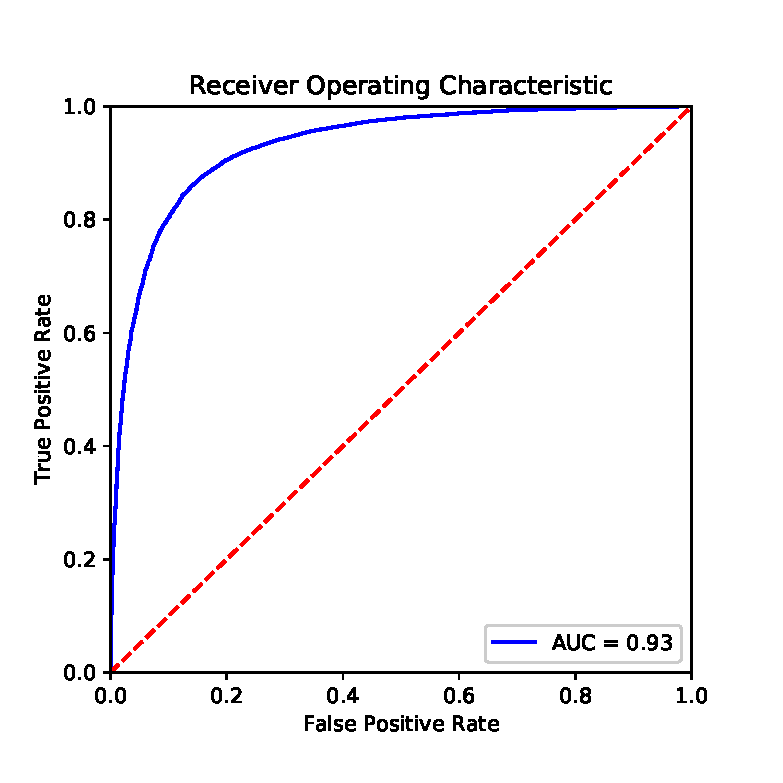
\includegraphics[width=0.4\linewidth]{figures/ch09_roccurve}
\caption{A ROC curve.}
\label{fig:roccurve}
\end{figure}

We can visualize this with a so-called ROC (reveicer operator
chraracteristic), a plot in which (Figure~\ref{fig:roccurve}) we plot
true positives against false positives at different thresholds.  A
good model extends until close to the upper left corner, and hence has
a large area under the curve (AUC).  If we choose a threshold at the
left end of the curve, we get little false positives (good!), but also
little true positives (bad!), if we go too far to the right, we get
the other extreme. So, how can we find the best spot?

One approach would be to print a table with three columns: the false
positive rate, the true positive rate, and the threshold value. You
then decide which FPR-TPR combination is most appealing to you, and
use the corresponding threshold value.

The second approach (also knwon as Yoden's J) is to find the threshold
value with the maximum distance between TPR and FPR, and use that one.

\todo[inline]{integrate code from https://github.com/damian0604/bdaca/blob/master/rm-course-2/week10/Determining\%20the\%20cutoff-point\%20in\%20logistic\%20regression.ipynb. But first look up how much space we actually have...}



\subsection{Train, test, validate}
By now, we have established which measures we can use to decide which
model to use. For all of them, we have assumed that we split our
labeled dataset into two: a training dataset and a test dataset. The
logic behind it was simple: If we would calculate precision and recall
on the training data itself, our assessment would be too optimistic --
after all, our models have been trained on exactly these data, so
predicting the label isn't too hard. Assessing the models on a different
dataset, the test dataset, instead, gives us an assessment of how
precision and recall look like if haven't seen the labels earlier --
which is exactly what we want to know.

Unfortunately, if we calculate precision and recall (or any other
metric) for multiple models on the same test dataset, and use these
results to determine which metric to use, we can run into a problem:
We may avoid overfitting of our model on the training data, we may now
overfit it on the test data! After all, we could tweak our models as
long until they fit our test data perfectly, even if this makes the
predictions for other cases worse.

One way to avoid this is to split the original data into three
datasets instead of two: a training dataset, a validation dataset, and
a test dataset.  We train multiple model configurations on the
training dataset and calculate the metrics of interest for all of them
on the validation dataset.  Once we have decided on a final model, we
calculate its performance (once) on the test dataset, to get an
unbiased estimate of its performance.



\subsection{Cross-validation and grid search}
\label{sec:crossvalidation}
In an ideal world, we would have a huge labelled dataset and do not
need to worry about the decreasing size of our training dataset as we
set aside our validation and test datasets.

Unfortunately, our labelled datasets in the real world have a limited
size, and setting aside too many cases can be problematic. Especially
if you are already on a tight budget, setting aside not only a test
dataset, but also a validation dataset of meaningful size may lead to
critically small training datasets. While we have addressed the
problem of overfitting, this could lead to underfitting: We may have
removed the only examples of some specific feature combination, for
instance.

A common approach to address this issue is $k$-fold
cross-validation. To do so, we split our data into $k$ partitions,
so-called folds. We then estimate our model $k$ times, and each time
leave \emph{one} of the folds aside for validation. Hence, every fold
is exactly one time the validation dataset, and exactly $k-1$ times
part of the training data. We then simply average the results of our
$k$ values for the evaluation metric we are interested in.

If our classifier generalizes well, we would expect that our metric of
interest (e.g., the accuracy, or the f1-score, \ldots) is very similar
in all folds. ~\refex{crossval} performs a cross-validation
based on the random forest classifier we build above. We see that,
even though there are no dramatic changes between the runs, there is
some variation. Running the same cross-validation on our logistic
regression classifier, instead, would produce not only better (higher)
means, but also better (lower) standard deviations.

\codex{chapter09/crossval.py}

Very often, cross-validation is used when we want to compare many
different model specifications, for example to find optimal
hyperparameters.

Hyperparameters are parameters of the model that are not estimated
from the data. These depend on the model, but could for example be the
estimation method to use, the number of times a bootstrap should be
repeated, etc. A very good example are the hyperparameters of support
vector machines (see above): It is hard to know how soft our margins
should be (the $C$), and we may also be unsure about the right kernel
(\refex{crossval2}), or in the case of a polinomial kernel, how many
degrees we want to consider).

Using the help function (e.g., \fn{RandomForestClassifier} in
Python or \fn{help(randomForest)} in R) or the documentation of the
modules you are using, you can look up which hyperparameters you can
specify. For a random forest classifier, for instance, this includes
the number of estimators in the model, the criterion, and whether or
not to use bootstrapping. \refex{gridsearch} illustrates how you can
automatically assess which values you should choose.

\codex{chapter09/gridsearch.py}

\codex{chapter09/gridsearch2.py}

\todo[inline]{Include examples in R for cross-validation.  Include crossval2 example, mentioned in the text. Comment the packages/functions used in examples crossval.py, crossval2.py,  gridsearch.py, gridsearch2.py}




\setcounter{chapter}{11}
\chapter{ Automatic analysis of text}
\label{chap:text}

In earlier chapters, you learned about both supervised and unsupervised machine learning as well about dealing with texts.
This chapter brings together these elements and discusses how to combine them to automatically analyze large corpora of texts. We begin with a very simple top-down approach in Section~\ref{sec:dictionary}, in which we count occurrences of words from an \emph{a priori} defined list of words. In Section~\ref{sec:supervised}, we still use pre-defined categories that we want to code, but let the machine ``learn'' the rules of the coding itself. Finally, in Section~\ref{sec:unsupervised}, we employ a bottom-up approach in which we do not use any \emph{a priori} defined lists or coding schemes, but inductively extract topics from our data.


\section{Dictionary approaches to text analysis}
\label{sec:dictionary}

A straightforward way to automatically analyze text is to compile a
list of terms you are interested in and simply count how often they
occur in each document. For example, if you are interested to find out
in how far mentions of political parties in news articles change over
the years, you only need to compile a list of all party names and
write a small script to count them.

Historically, this is how sentiment analysis was
done. \refex{sentsimple} shows how to do a simple sentiment analysis
based on a list of positive and negative words. The logic is
straightforward: you count how often each positive word occurs in a
text, you do the same for the negative words, and then determine which
occur more often.

\todo[inline]{The example now shows two very differnet approaches. We probably could find a NLTK function or sth to make the python-example more R-like ... but on the other hand, it seems (but maybe that's me (Damian)) more flexible and extensible to build this up as a for loop, especially if you eventually want to support multi-word expressions or regex or so. TO BE DECIDED...}


\pyrex[input=both, output=none, caption={Different approaches to a simple dictionary-based sentiment analysis: counting and summing all words using a for-loop over all reviews (Python) versus constructing a term-document matrix and looking up the words in there (R). Note that both approaches would be possible in either language.}]{chapter12/sentsimple}

As you may already realize, there are a lot of downsides to this
approach. Most notably, our bag-of-words approach does not allow us to
allow for negation: ``not good'' will be counted as
positive. Relatedly, we cannot handle modifiers such as ``very
good''. Also, all words are either positive or negative, while
``great'' should be more positive than ``good''. More advanced
dictionary-based sentiment analysis packages like \cite{vader},
\cite{sentistrength} include such functionality. Yet, as we will
discuss in Section~\ref{sec:supervised}, also these off-the-shelf
packages perform very poorly in many sentiment analysis tasks.

Still, there are many use cases where dictionary approaches work very
well. Because your list of words can contain anything, not just
positive or negative words. Dictionary approaches have been used, for
instance, to measure the use of racist words or swearwords in online
fora. Dictionary approaches are simple to understand and
straightforward, which can be a good argument for using them when it
is important that the method is no black-box but fully transparent
even for a layperson. Especially when the dictionary is already
existing or easy to create, it is also a very cheap method. This goes
at the expense, though, of their limitation to measuring easy to
operationalize concepts. To put it bluntly: it's great for measuring
the visibility of parties or organizations in the news, but it's not
good for measuring frames.

What gave dictionary approaches a bit of a bad name is that many
researchers applied them without validating them. This is especially
problematic when a dictionary is applied in a slightly different
domain than for which it was originally made.

If you want to use a dictionary-based approach, we advise the
following procedure:

\begin{enumerate}
  \item Construct a dictionary based on theoretical considerations and by closely reading a sample of example texts.
  \item Code some articles manually and compare with the automated coding.
  \item Improve your dictionary and check again.
  \item Manually code a validation dataset of sufficient size. The required size depends a bit on how balanced your data is -- if one code occurs very infrequently, you will need more data.
  \item Calculate the agreement. You could use standard intercoder reliability measures used in manual content analysis, but we would also advise you to calculate precision and recall (see Secion~\ref{sec:validation}).
  \end{enumerate}

Very extensive dictionaries will have a high recall (it becomes
increasingly unlikely that you ``miss'' a relevant document), but
often suffer from low precision (more documents will contain one of
the words even though they are irrelevant). Vice versa, a very short
dictionary will often be very precise, but miss a lot of documents.
It depends on your research question where the right balance lies, but
to substantially interpret your results, you need to be able to
quantify the performance of your dictionary-based approach.


\section{Supervised text analysis: automatic classification and sentiment analysis}
\label{sec:supervised}

For many applications, there are good reasons to use the dictionary
approach presented in the previous section. First, it is intuitively
understandable and results can -- in principle --
even be varified by hand, which can be an advantage when transparency
or communicatibility is of high importance. Second, it is very easy to
use.

%TODO hoort deze beschrijving niet bij 12.1? (of 12.0, of een aparte sectie `choosing a method')?
Dictionary approaches excel under three conditions: First, the
variable we want to code is \emph{manifest and concrete} rather than
\emph{latent and abstract}: names of actors, specific physical
objects, specific phrases, etc., rather than feelings, frames, or
topics. Second, all synonyms to be included must be known
beforehand. And third, the dictionary entries must not have multiple
meanings.

For instance, coding how often gun control is mentioned in political
speeches fits these criteria. There are only so many ways to talk
about it, and it is rather unlikely that speeches about other topics
contain a phrase like ``gun control''. Similarly, if we want to find
references to Angela Merkel, Donald Trump, or any other well-known
politician, we can just directly search for their names -- even though
problems arise when people have very common surnames and are referred
to by their surnames only.

Sadly, most interesting concepts are more complex to code. Take a
seemingly straightforward problem: distinguishing whether a news
article is about the economy or not. This is really easy to do for
humans: there may be some edge cases, but in general, people rarely
need longer than a few seconds to grasp whether an article is about the
economy rather than about sports, culture, etc. Yet, many of these
articles won't directy state that they are about the economy by
explicitly using the word ``economy''.

We may think of extending our dictionary not only with |economi.*| (a
regular expression that includes economists, economic, and so on), but
also come up with other words like ``stock exchange'', ``market'',
``company.'' Unfortunately, we will quickly run into a problem that we also
faced when we dicussed the precision-recall tradeoff in
Section~\ref{sec:validation}: The more terms we add to our
dictionary, the more false positives we will get: articles about
the geographical space called ``market'', about some celebrity being seen
in ``company'' of someone else, and so on.

From this example, we can conclude that often (1) it is easy for
humans to decide to which class a text belongs, but (2) it is very
hard for humans to come op with a list of words (or rules) on which
their judgement is based.

Such a situation is perfect for applying supervised machine
learning: After all, it won't take us much time to annotate, say, 1000
articles based on whether they are about the economy or not (probably
this takes less time than thoroughly finetuning a list of words to in-
or exclude); and the difficult part, deciding on the exact rules
underlying the decision to classify an article as economic is done by
the computer in seconds.


\subsection{Putting together a workflow}
\label{sec:workflow}

With the knowledge we gained in previous chapters, it is not difficult
to set up a supervised machine learning classifier to automatically
determine, for instance, the topic of a news article.

Let us recap the building blocks that we need. In
Chapter~\ref{chap:introsml}, you learned how to use different
classifiers, how to evaluate them, and how to choose the best
settings. However, in these examples, we used numerical data as
features; now, we have text.  In \refchap{dtm},
you learned how to turn text into numerical
features. And that's all we need to get started!

Typical examples for supervised machine learning in the analysis of
communication include the classification of topics
\citep[e.g.,][]{Scharkow2011}, frames \citep[e.g.,][]{Burscher2014},
user characteristics such as gender or ideology,
or sentiment.

Let us consider the case of sentiment analysis more in
detail. Classical sentiment analysis is done with a dictionary
approach: you take a list of positive words, a list of negative words,
and count what occurs more. Addtionally, one may attach a weight to
each word, such that ``perfect'' gets a higher weight than ``good'',
for instance.  An obvious drawbacks is that these pure
bag-of-words approaches cannot cope with negation (``not good'') and
intensifiers ``very good''), which is why extensions have been
developed that take these (and other features, such as punctuation)
into accout \citep{Thelwall2012,Hutto2014,DeSmedt2012}.
% come back to this in crowddcoding-chapter: \citep{Haselmayer2016}

But while available off-the-shelf packages that implement these
extended dictionary-based methods are very easy to use (in fact, they
spit out a sentiment score with one single line of code), it is
questionable how well they work in practice. After all, ``sentiment''
is not exactly a clear, manifest concept for which we can enumerate a
list of words. It has been shown that results obtained with multiple
of these packages correlate very poorly with each other and with human
annotations \citep{Boukes2019,Chan2021}.

Consequently, it has been suggested that it is better to use
supervised machine learning to automatically code the sentiment of
texts \citep{Gonzalez-Bailon2015,vermeer2019seeing}. In particular,
one may need to annotate a custom, own dataset: training a classifier
on, for instance, movie reviews and then using it to predict sentiment
in political texts violates the assumption that training set, test
set, and the unlabeled data that are to be classified are (at least in
principle and approximately) drawn from the same population.

To illustrate the workflow, we will use the ACL IMDB dataset, a large
dataset that consists out of a training dataset of 25,000 movie
reviews (out of which 12,500 positives ones and 12,500 negative ones)
and an equally sized test dataset \citep{aclimdb}. It can be
downloaded at
\url{https://ai.stanford.edu/~amaas/data/sentiment/aclImdb_v1.tar.gz}


These data do not come in one file, but rather in a set of textfiles
that are sorted in different folders named after the dataset they
belong to (|test| or |train|) and their label (|pos| and |neg|). This
means that we cannot simply use a pre-defined function to read them,
but we need to think of a way of reading the content into a
datastructure that we can use. One way of doing so is shown in
\refex{readimdb}.

\pyrex[output=none, caption={Reading the ACL IMDB dataset.}]{chapter12/readimdb}

\label{feature:sparse}
\begin{feature}
  \textbf{Sparse versus dense matrices and why it matters a lot for
    choosing between R and Python for machine learning.} In a
  document-term matrix, you would typically find a lot of zeros: most
  words do \emph{not} appear in any given document. For instance, the
  reviews in the IMDB dataset contain more than 100,000 unique
  words. Hence, the matrix has more than 100,000 columns. Yet, most
  reviews only consist of a couple of hundreds of words. As a
  consequence, more than 99\% of the cells in the table contain a
  zero. In a sparse matrix, we do not store all these zeros, but only
  store the values for cells that actually contain a value. This
  drastically reduces the memory needed.  But even if you have a huge
  amount of memory, this does not solve the issue: In R, the number of
  cells in a matrix is limited to 2,147,483,647. It is therefore
  impossible to store a matrix with 100,000 features and 25,000
  documents as a dense matrix. Unfortunately, many models that you can
  run via \pkg{caret} in R will convert your sparse document-term
  matrix to a dense matrix, and hence are effectively only usable for
  very small datasets. An alternative is using the \pkg{quanteda} package,
  which does use sparse matrices throughout. However, at the time of
  writing this book, quanteda only provides a very limited number of
  models. As all of these problems do not arise in \pkg{scikit-learn},
  you may want to consider using Python for many text classification tasks.
\end{feature}


Let us now train our first classifier. We choose a Na\"ive Bayes
classifier with a simple count vectorizer (\refex{imdbbaseline}).  In
the Python example, pay attention to the fitting of the vectorizer: we
fit on the training data \emph{and} transform the training data with
it, but we only transform the test data \emph{without re-fitting the
  vectorizer}. Fitting, here, includes the decision which words to
include (by definition, words that are not present in the training
data are not included; but we could also choose additional
constraints, such as excluding very rare or very common words), but
also assigning an (internally used) identifier (variable name) to each
word. If we would fit the classifier again, these would not be
compatible any more. In R, the same is achieved in a slightly
different way: Two term-document matrices are created independently,
before they are matched in such a way that only the features that are
present in the training matrix are retained in the test matrix.


\note{A word that is not present in the training data, but is present
  in the test data, is thus ignored. If you want to use the
  information such out-of-vocabulary words can entail (e.g., they may
  be synonyms), you need to use a word embedding approach (see \refsec{wordembeddings})}

We do not necessarily expect this first model to be the best
classifier we could come up with, but it provides us with a reasonable
baseline. In fact, even without any further adjustments, it works
reasonably well: precision is higher for positive reviews and recall
is higher for negative reviews (classifying a positive review as
negative happens twice as much as the reverse), but none of the values
is concerningly low.

\pyrex[output=py, caption=Training a Na\"ive Bayes classifier with simple word counts as features]{chapter12/imdbbaseline}



\subsection{Finding the best classifier}

%\todo[inline]{\url{https://github.com/quanteda/quanteda.textmodels} seems to be under heavy development right now. In the CRAN version of quanteda, there is only a NB classifier present. Let's wait for a moment to check which textmodels will be available via quanteda and then incorporate them here.}
% As of 2020-11-10, still only logreg, svm, nb -- better, but much less than scikit lean


%TODO: Beter uitleggen (+ref ch 11)
Let us start by comparing two simple classifiers we know (Na\"ive
Bayes and Logistic Regression (see Section~\ref{sec:nb2dnn}) and two
vectorizers that transform our texts into two numerical
representations that we know: word counts and $tf\cdot idf$ scores
(see \refchap{dtm}).

We can also tune some things in the vectorizer, such as filtering out
stopwords, or specifying a minimum number (or proportion) of documents
in which a word needs to occur in order to be included, or the maximum
number (or proportion) of documents in which it is allowed to
occur. For instance, it could make sense to say that a word that
occurs in less than $n=5$ documents is probably a spelling mistake or
so unusual that it just unnecessarily bloats our feature matrix; and
on the other hand, a word that is so common that it occurs in more
than 50\% of all documents is so common that it does not help us to
distinguish between different classes.

We can try all of these things out by hand by just re-running the code
from \refex{imdbbaseline} and only changing the line in which the
vectorizer is specified and the line in which the classifier is
specified.
However, copy-pasting essentially the
same code is generally not a good idea, as it makes your code unnecessary
long and increases the likelihood of errors creeping in when you, for
instance, need to apply the same changes to multiple copies of the
code.  A more elegant approach is outlined in
\refex{basiccomparisons}: We define a function that gives us a short
summary of only the output we are interested in, and then use a
for-loop to iterate over all configurations we want to evaluate, fit
them and call the function we defined before. In fact, with 23 lines
of code, we manage to compare four different models, while we already
needed 15 lines (in \refex{imdbbaseline}) to evaluate only one model.


%TODO R-code?
\pyrex[input=py, output=py, caption={An example of a custom function to give a brief overview of the performance of four simple vectorizer-classifier combinations.}]{chapter12/basiccomparisons}


The output of this little example gives us already quite a bit of
insight into how to tackle our specific classification tasks: First, we
see that a $tf\cdot idf$ classifier seems to be slightly but
consistently superior to a count classifier (this is often, but not
always the case). Second, we see that the logistic regression performs
better than the Na\"ive Bayes classifier (again, this is often, but not
always, the case). In particular, in our case, the logistic regression
improved on the excessive misclassifcation of positive reviews as
negative, and achieves a very balanced performance.

There may be instances where one nevertheless may want to use a Count
Vectorizer with a Na\"ive Bayes classifier instead (especially if it
is too computationally expensive to estimate the other model), but for
now, we may settle on the best performing combination, logistic
regression with a $tf\cdot idf$ vectorizer. You could also try fitting
a Support Vector Machine instead, but we have little reason to believe
that our data isn't linearly separable, which means that there is
little reason to believe that the SVM will perform better. Given the
good performance we already achieved, we decide to stick to the
logistic regression for now.


We can now go as far as we like, include more models, use
crossvalidation and gridsearch (see
Section~\ref{sec:crossvalidation}), etc. However, our workflow now
consists of \emph{two} steps: fitting/transforming our input data
using a vectorizer, and fitting a classifier. To make things easier,
in scikit-learn, both steps can be combined into a so-called
pipe. \refex{basicpipe} shows how the loop in
\refex{basiccomparisons} can be re-written using pipes (the
result stays the same).

\pyrex[input=py, output=none, caption={Instead of fitting vectorizer and classifier separately, they can be combined in a pipeline.}]{chapter12/basicpipe}

Such a pipeline lends itself very well for performing a
gridsearch. \refex{gridsearchlogreg} gives you an example.  With
|LogisticRegression?| and |TfIdfVectorizer?|, we can get a list of all
possible hyperparameters that we may want to tune. For instance, these
could be the minimum and maximum frequency for words to be included or
whether we want to use only unigrams (single words) or also bigrams
(combinations of two words, see \refsec{ngram}.
For the Logistic Regression, it may be the
regularization hyperparameter C, which applies a penalty for too
complex models.  We can  put all values for these parameters
that we want to consider in a dictionary, with a descriptive key (i.e., a string with the step of the pipeline followed by two underscores and the name of the hyperparameter) and a list of all values we want to consider as corresponding value.

The gridsearch procedure will then estimate all combinations of all
values, using cross-validation (see Section~\ref{sec:validation}). In
our example, we have $2 \cdot 2 \cdot 2 \cdot 2 \cdot 3 = 24$
different models, and $24$ models $\cdot 5$ folds $= 120$ models to
estimate. Hence, it may take you some time to run the code.

\pyrex[input=py, output=py, caption={A gridsearch to find the best hyperparameters for a pipeline consisting of a vectorizer and a classifier. Note that we can tune any parameter that either the vectorizer or the classifier accepts as an input, not only the four hyperparameters we chose in this example.}]{chapter12/gridsearchlogreg}

We see that we could further improve our model to precision and recall
values of .90, by excluding extremely infrequent and extremely
frequent words), including both unigrams and bigrams (which, we may
speculate, helps us accounting for the ``not good'' vs ``not'',
``good'' problem), and changing the default penalty of C=1 to C=100.

Let us, just for the sake of it, compare the performance of our model
with an off-the-shelf sentiment analysis package, in this case Vader
\citep{Hutto2014}. For any text, it will directly estimate sentiment
scores (more specifically, a positivity score, a negativity score, a
neutrality score, and a compound measure that combines them), without
any need to have training data. However, as \refex{vader} shows, such
a method is clearly inferior to a supervised machine learning
approach. While in almost all cases (except for $n=11$ cases), Vader was able to
make a choice (getting scores of 0 is a notorious problem in very
short texts), precision and recall are clearly worse than even the
simple baseline model we started with, and much worse than those of
the final model we finished with. In fact, we miss half (!) of the
negative reviews. There are probably very few applications in the
analysis of communication in which we would find this acceptable.
It is important to highlight that this is not because the off-the-shelf
package we chose is a particularly bad one (on the contrary, it is
actually comparatively good), but because of the inherent limitations
of dictionary-based sentiment analysis.

\pyrex[input=py, output=py, caption={For the sake of comparison, we calculate how an off-the-shelf sentiment analysis package would have performed in this task}]{chapter12/vader}

We need to keep in mind, though, that with this dataset, we chose one
of the easiest sentiment analysis tasks: a set of long, rather formal
texts (compared to informal short social media messages), that
evaluate exactly one entity (one film), and that are not ambigous at
all. Many applications that communication scientists are interested
in are much less straight-forward. Therefore, however tempting it may be
to use an off-the-shelf package, doing so requires a thorough test
based on at least some human-annotated data.



\subsection{Using the model}

So far, we have focused on training and evalualting models, almost
forgetting why we were doing this in the first place: to use them to
predict the label for new data that we did not annotate.

Of course, we could always re-train the model when we need to use it
-- but that has two downsides: first, as you may have seen, it may
actually take considerable time to train it, and second, you need to
have the training data available, which may be a problem both in terms
of storage space and of copyright and/or privacy if you want to share
your classifier with others.

Therefore, it makes sense to save both our classifier and our
vectorizer to a file, so that we can reload them later
(\refex{reuse}). Keep in mind that you have to re-use \emph{both}
-- after all, the columns of your feature matrix will be different (and hence, completely useless for the classifier) when
fitting a new vectorizer. Therefore, as you see, you do not do any fitting any more, and only use the |.transform()| method of the (already fitted) vectorizer and the |.predict()| method of the (already fitted) classifier.

In R, you have no vectorizer you could save -- but because in contrast to Python, both your DTM and your classifier include the feature names, it suffices to save the classifier only (using \verb+saveRDS(myclassifier, "myclassifier.rds")+) and using on a new DTM later on. You do need to remember, though, how you constructed the DTM (e.g., which preprocessing steps you took), to make sure that the features are comparable.

\pyrex[output=py, input=py, caption=Saving and loading a vectorizer and a classifier]{chapter12/reuse}



Another thing that we might want to do is to get a better idea of the
features that the model uses to arrive at its prediction; in our
example, what actually characterizes the best and the worst
reviews. \refex{eli5} shows how this can be done in one line of code
using \pkg{eli5} -- a package that aims to ``\emph{e}xplain [the model]
\emph{l}ike \emph{I}'m \emph{5} years old''. Here, we re-use the
|pipe| we constructed earlier to provide both the vectorizer and the
classifier to the eli5 -- if we would have only provided the
classifier, then the feature names would have been internal
identifiers (which are meaningless to us) rather than human-readable
words.

\pyrex[output=py, format=html, caption=Using ELI5 to get the most predictive features]{chapter12/eli5}

We can also use eli5 to explain how the classifier arrived at a
prediction for a specific document, by using different shades of green
and red to explain how much different features contributed to the
classification, and in which direction (\refex{eli5b}).

\pyrex[output=py, input=py, format=html, caption=Using ELI5 to explain a prediction]{chapter12/eli5b}


\todo[inline]{Include an example of RNN to text classification}



\section{Unsupervised text analysis: topic modeling}
\label{sec:unsupervised}

In \refsec{clustering}, we discussed how clustering techniques can be used to find patterns in data,
such as which cases or respondents are most similar.
Similarly, especially in survey research it is common to use factor analysis to discover (or confirm) variables that form a scale.

In essence, the idea behind these techniques is similar:
by understanding the regularities in the data (which cases or variables behave similarly),
you can describe the relevant information in the data with fewer data points.
Moreover, assuming the regularities capture interesting information and the deviations from these regularities are mostly
uninteresting noise, these clusters of cases or variables can actually be substantively informative.

Since a document-term matrix (DTM) is `just' a matrix, you can also apply these clustering techniques to the DTM
to find groups of words or documents. You can therefore use any of the techniques we described in \refchap{eda}, and in particular clustering techniques such as $k$-means clustering (see  \refsec{clustering}) to group documents that use similar words together. 

It can be very instructive to do this, and we encourage you to play around with such techniques. However, in recent years, a set of models called \concept{topic models} have become especially popular for the unsupervised analysis of texts. Very much what like what you would do with other unsupervised techniques, also in topic modeling, you group words and documents into `topics', consisting of words and documents that co-vary.
If you see the word `agriculture' in a news article, there is a good chance you might find words such as `farm' or `cattle',
and there is a lower chance you will find a word like `soldier'.
In other words, the words `agriculture' and `farm' generally occur in the same kind of documents, so they can be said to be part of the same topic.
Similarly, two documents that share a lot of words are probably about the same topic,
and if you know what topic a document is on (e.g. an agricultural topic), you are better able to guess what words might occur in that document (e.g. `cattle')

Thus, we can formulate the goal of topic modeling as: given a corpus, find a set of N topics, consisting of specific words and/or documents, that minimize the mistakes we would make if we try to reconstruct the corpus from the topics.
This is similar to regression where we try to find a line that minimizes the prediction error.

In early research on document clustering, a technique called Latent Semantic Analysis (LSA) essentially used a factor analysis technique called Singular Value Decomposition (see \refsec{pcasvd}) on the DTM.
This has yielded promising results in information retrieval (i.e. document search) and studying human memory and language use.
However, it has a number of drawbacks including factor loadings that can be difficult to interpret substantively and no good way of dealing with words that can have multiple meanings \citep{lsa}.

\subsection{Latent Dirichlet Allocation (LDA)}

The most widely used technique for topic modeling is Latent Dirichlet Allocation (LDA).
Although the goal of LDA is the same as for clustering techniques, it starts from the other end with what is called a \concept{generative model}.
A generative model is a (simplified) formal model of how the data is assumed to have been generated.
For example, if we would have a standard regression model predicting income based on age and education level,
the implicit generative model is that to determine someone's income, you take their age and education level,
multiply them both by their regression parameters, and then add the intercept and some random error.
Of course, we know that's not actually how most companies determine wages, but it can be a useful starting point to analyze e.g. labour market discrimination.

The generative model behind LDA works as follows.
Assume that you are a journalist writing a 500 word news item.
First, you would choose one or more \emph{topics} to write about,
for example 70\% healthcare and 30\% economy.
Next, for each word in the item, you randomly pick one of these topics based on their respective weight.
Finally, you pick a random word from the words associated with that topic,
where again each word has a certain probabibility for that topic.
For example, `hospital' might have a high probability for healthcare while `effectiveness' might have a lower probability but could still occur.

As said, we know (or at least strongly suspect) that this is not how journalists actually write their stories.
However, this generative model helps understand the substantive interpretation of topics.
Moreover, LDA is a \concept{mixture model}, meaning it allows for each document to be about multiple topics, and for each word to occur in multiple topics.
This matches with the fact that in many cases, our documents are in fact about multiple topics,
from a news article about the economic effects of the COVID virus to an open survey answer containing multiple reasons for supporting a certain candidate. 
Additionally, since topic assignment is based on what other words occur in a document,
the word `pupil' could be assigned either to a `biology' topic or to an `education' topic, depending
on whether the document talks about eyes and lenses or about teachers and classrooms.

\begin{figure}
  \includegraphics[width=\linewidth]{chapter12/lda.png}
  \caption{Latent Dirichlet Allocation in `Plate Model' notation \citep[fig. 1]{blei03}}\label{fig:lda}
\end{figure}

\reffig{lda} is a more formal notation of the same generative model.
Starting from the left, for each document you pick a set of topics $\Theta$.
This set of topics is drawn from a \concept{Dirichlet distribution} which itself has a parameter $\alpha$
(see note).
Next, for each word you select a single topic $z$ from the topics in that document.
Finally, you pick an actual word $w$ from the words in that topic, again controlled by a paramter $\beta$ (see note).

Now, if we would know which words and documents are in which topics, we could start generating the documents in the corpus.
In reality, of course, we have the reverse situation:
we know the documents, and we want to know the topics.
Thus, the task of LDA is to find the parameters that have the highest chance of generating these documents.
Since only the word frequencies are observed, this is a latent variable model where we want to find the
most likely values for the (latent) topic $z$ for each word in each document. 

Unfortunately, there is no simple analytic solution to calculate these topic assignments
like there is for OLS regression.
Thus, like other more complicated statistical models such as multilevel regression,
we need to use an iterative estimation that progressively optimizes the assignment to improve the fit until it converges.

An estimation method that is often used for LDA is Gibbs sampling.
Simply put, this starts with a random assignment of topics to words.
Then, each iteration, it reconsiders each words and recomputes what likely topics for that word are
given the other topics in that document and the topics that word occurs in  other documents.
Thus, if a document already contains a number of words placed in a certain topic,
a new word is more likely to be placed in that topic as well.
After enough iterations, this converges to a solution. 

\note{\textbf{The Dirichlet Distribution and its Hyperparameters}
  The Dirichlet distribution can be seen as a distribution over multinomial distributions,
  that is, every draw from a dirichlet distribution results in a multinomial distribution.
  An easy way to visualize this is to see the dirichlet distribution as a bag of dice.
  You draw a die from the bag, and each die is a distribution over the numbers one to six.

  This distribution is controlled by a parameter called alpha ($\alpha$),
  which is often called a \concept{hyperparameter} because it is a parameter that controls how other parameters
  (the actual topic distributions) are estimated, similar to e.g. the learning speed in many machine learning models.
  This alpha hyperparameter controls what kind of dice there are in the bag.
  A high alpha means that the dice are generally fair, i.e., give a uniform multinomial distribution.
  For topic models, this means that documents will in general contain an even spread of multiple topics.
  A low alpha means that each die is unfair in the sense of having a strong preference for some number(s), as if these numbers are weighed down. You can then draw a die that prefers ones, or a die that prefers sixes.
  For topic models this means that each document tends to have one or two dominant topics.
  Finally, alpha can be symmetric (meaning dice are unfair, but randomly, so in the end each topic has the same chance)
  or asymetric (they are still unfair, and now also favour some topics more than others).
  This would correspond to some topics being more likely to occur in all documents.
  
  In our experience, most documents actually do have one or two dominant topics,
  and some topics are actually more prevalent across many documents then others
  -- especially if you consider that procedural words and boilerplate also need to be fit into a topic unless they are filtered out beforehand.
  Thus, we would generally recommend a relatively low and asymmetric alpha,
  and in fact \pkg{gensim} provides algorithm to find, based on the data, an alpha that corresponds to this recommendation (by specifying \texttt{alpha='auto'}).
  In R, we would recommend picking a lower alpha than the default value, probably around $\alpha=5/K$,
  and optionally try using an asymmetric alpha if you find some words that occur across multiple topics. 

  To get a more intuitive understanding of the effects of alpha,
  please see \url{http://cssbook.net/lda} for additional material and visualizations.
  }

\subsection{Fitting an LDA model}


\begin{ccsexample}
\doublecodex{chapter12/lda1}
\codex[caption=Output (from R)]{chapter12/lda1.r.out}
\doublecodex{chapter12/lda2}
\codexoutputtable{chapter12/lda2.r}
\caption{LDA Topic Model of Obama's State of the Union speeches}\label{ex:lda}
\end{ccsexample}

\refex{lda} shows how you can fit an LDA model in Python or R.
As example data, we use Obama's State of the Union Speeches using the corpus introduced in \refchap{dtm}.
Since such a speech generally touches on many different topics, we choose to first split by paragraph
as these will be more semantically coherent (for Obama, at least).
In R, we use the \fn{corpus\_reshape} function to split the paragraphs,
while in Python we use \pandas' \fn{str.split}, which creates a list or paragraphs for each text,
which we then convert into a paragraph per row using \fn{explode}.
Converting this to a DTM we get a reasonably sized matrix of 738 paragraphs and 746 unique words.

Next, we fit the actual LDA model using the package \pkg{gensim} (Python) and \pkg{topicmodels}.
Before we can do this, we need to convert the DTM format into a format accepted by that package.
For Python, this is done using the \fn{Sparse2Corpus} helper function while in R this is done with the \quanteda\ \fn{convert} function.
Then, we fit the model, asking for 10 topics to be identified in these paragraphs.
There are three things to note in this line.
First, we specify a \concept{random seed} of 123 to make sure the analysis is replicable.
Second, we specify an `asymmetric' of \verb|1/1:10|, meaning the first topic has alpha 1, the second 0.5, etc (in R).
In Python, instead  of using the default of \verb|alpha='symmetric'|, we set  \verb|alpha='asymmetric'|, which uses the formula
$\frac{1}{topic\_index + \sqrt{num\_topics}}$ to determine the priors. At the cost of a longer estimation time, we can even
specify \verb|alpha='auto'|, which will learn an asymetric prior from the data. For more background, see the note on hyperparameters for more information. 
Third, for Python we also need to specify the vocabulary names since these are not included in the DTM.

The final line generates a data frame of top words per topic for first inspection
(which in Python requires separating the words from their weights in a list comprehension and converting it to a dataframe for easy viewing).
As you can see, most topics are interpretable and somehwat coherent: For example, topic 1 seems to be about education and jobs,
while topic two is health care. You also see that the word `job' occurs in multiple topics (presumably because unemployment was a pervasive concern during Obama's tenure).
Also, some topics like topic 3 are relatively more difficult to interpret from this table.
A possible reason for this is that not every paragraph actually has policy content.
For example, the first paragraph of his first State of the Union was:
\emph{`Madam Speaker, Mr. Vice President, Members of Congress, the First Lady of the United States -- she's around here somewhere'}.
None of these words really fit a `topic' in the normal meaning of that term,
but all of these words need to be assigned a topic in LDA.
Thus, you often see `procedural' or `boilerplate' topics such as topic 3 occurring in LDA outputs. 

Finally, note that we showed the R results here. As \pkg{gensim} uses a different estimation algorithm
(and \sklearn\ uses a different tokenizer and stopword list), results will not be identical,
but should be mostly similar. 

\subsection{Analyzing topic model results}

\begin{ccsexample}
\doublecodex{chapter12/ldaresults1}
\codexoutputtable{chapter12/ldaresults1.r}
\doublecodex{chapter12/ldaresults2}
\codex[caption=Output (from R)]{chapter12/ldaresults2.r.out}
\caption{Analyzing and inspecting LDA results}\label{ex:ldaresults}
\end{ccsexample}


\refex{ldaresults} shows how you can combine the LDA results (topics per document)
with the original document metadata.
This could be your starting point for substantive analyses of the results,
for example to investigate relations between topics or between e.g. time or partisanship and topic use.

You can also use this to find specific documents for reading.
For example, we noted above that topic 3 is difficult to interpret.
As you can see in the table in \refex{ldaresults} (which is sorted by value of topic 3),
most of the high scoring documents are the first paragraph in each speech,
which do indeed contain the ``Madam speaker'' boilerplate noted above.
The other three documents are all calls for bipartisanship and support.
As you can see from this example, carefully inspecting the top documents for each topic
is very helpful for making sense of the results.


\subsection{Validating and inspecting topic models}

As we saw in the previous subsection, running a topic model is relatively easy.
However, that doesn't mean that the resulting topic model will always be useful.
As with all text analysis techniques, \concept{validation} is the key to good analysis:
are you measuring what you want to measure? And how do you know?

For topic modeling (and arguably for all text analysis),
the first step after fitting a model is inspecting the results and establishing face validity.
Top words per topic such as listed above are a good place to start with this,
but we would really encourage you to also look at the top documents per topic to better understand how words are used in context.
Also, it is good to inspect the relations between topics and look at documents that load high on multiple topics to understand the relation.

If the only goal is to get an explorative understanding of the corpus,
for example as a first step before doing a dictionary analysis or manual coding,
just face validity is probably sufficient.
For a more formal validation, however, it depends on the reason for using topic modeling.

If you are using topic modeling in a true unsupervised sense, i.e. without a predefined analytic schema in mind,
it is difficult to assess whether the model measures what you want to measure --
because the whole point is that you don't know what you want to measure.
That said, however, you can have the general criteria that the model needs to achieve \emph{coherence}
and \emph{interpretability}, meaning that words and documents that share a topic
are also similar semantically. 

In their excellent paper on the topic, \citet{chang09} propose two formal tasks to judge this
using manual (or crowd) coding: in \emph{word intrusion}, a coder is asked to pick the `odd one out' from a list
where one other word is mixed in a group of topic words.
In \emph{topic intrusion}, the coder is presented with a document and a set of topics that occur in the document,
and is asked to spot the one topic that was not present according to the model.
In both tasks, if the coder is unable to identify the intruding word or topic, apparently the model does not fit
our intuitive notion of `aboutness' or semantic similarity.
Perhaps their most interesting finding is that goodness-of-fit measures like perplexity\footnote{Perplexity is measure to compare and evaluate topic models using log-likelihood in order to estimate how well a model predicts a sample.} 
are actually not good predictors of the interpretability of the resulting models.

If you are using topic models in a more confirmatory manner,
that is, if you wish the topics to match some sort of predefined categorization,
you should use regular gold standard techniques for validation:
code a sufficiently large random sample of documents with your predefined categories,
and test whether the LDA topics match those categories.
In general, however, in such cases it is a better idea to use a dictionary or supervised analysis technique
as topic models often do not exactly capture our categories. After all, unsupervised techniques mainly
excel in bottom-up and explorative analyses (\refsec{deciding}).


\subsection{Beyond LDA}

This chapter focused on regular or `vanilla' LDA topic modeling.
Since the seminal publication, however, a large amount of variations and extensions on LDA have been proposed.
These include, for example, dynamic topic models (which incorporate time; \cite*{dynamiclda}),
correlated topic models (which explicitly model correlation between topics; \cite{correlatedlda}).
Although it is beyond the scope of this book to describe these models in detail,
the interested reader is encouraged to learn more about these models.

Especially noteworthy are \concept{Structural Topic Models} (R package \pkg{stm}; \cite*{stm}),
which allow you to model covariates as topic or word predictors.
This allows you, for example, to model topic shifts over time or
different words for the same topic based on e.g. Republican or Democrat presidents. 

Python users should check out Hierarchical Topic Modeling \citep{hierarchicallda}.
In hierarchical topic modeling, rather than the researcher specifying a fixed number of topics,
the model returns a hierachy of topics from few general topics to a large number of specific topics,
allowing for a more flexible exploration and analysis of the data. 






\backmatter
% bibliography, glossary and index would go here.

\begin{small}
\printbibliography
\end{small}


\end{document}
